\documentclass[a4paper,fleqn]{cas-sc}

% =========================================================
% PACKAGES
% =========================================================

\usepackage[numbers]{natbib}
\usepackage{graphicx}
\usepackage{amsmath,amssymb}
\usepackage{booktabs}
\usepackage{multirow}
\usepackage{array}
\usepackage{siunitx}
\usepackage{xcolor}
\usepackage[left]{lineno}

% =========================================================
% REMOVE ELSEVIER CAS PREPRINT FOOTER FROM ALL PAGES
% =========================================================

\ExplSyntaxOn
\cs_set:Npn \__first_foot: { }
\cs_set:Npn \__cas_foot: { }
\csname ps@cas\endcsname
\ExplSyntaxOff

% =========================================================
% DOCUMENT
% =========================================================

\begin{document}

% Continuous line numbering in left margin
\linenumbers

\let\WriteBookmarks\relax
\def\floatpagefraction{1}
\def\textpagefraction{.001}

% =========================================================
% FRONT MATTER
% =========================================================

\shorttitle{Multi-Objective Optimisation for Battery Forecasting}

\shortauthors{Simhaa T. T. and Sivakumar B.}

\title[mode=title]
{Multi-Objective Evolutionary Hyperparameter Optimisation for Recursive Battery Degradation Forecasting}

% =========================================================
% AUTHORS AND AFFILIATIONS
% =========================================================

\author[1]{Simhaa T. T.}[
    orcid=0009-0006-9041-1103
]

\author[2]{Sivakumar B.}[
    orcid=0000-0002-3612-6241
]

\affiliation[1]{
    organization={Department of Electrical and Electronics Engineering,
    Sri Sivasubramaniya Nadar College of Engineering},
    city={Chennai},
    state={Tamil Nadu},
    country={India}
}

\affiliation[2]{
    organization={Department of Mathematics,
    Sri Sivasubramaniya Nadar College of Engineering},
    city={Chennai},
    state={Tamil Nadu},
    country={India}
}

% =========================================================
% ABSTRACT
% =========================================================

\begin{abstract}
Under a matched budget of 280 candidate evaluations per run, NSGA-II achieved a final mean hypervolume of 1.1972, exceeding NSGA-III (1.1579; Holm-corrected $p = 2.7\times10^{-4}$) and random search (1.1410; $p = 1.2\times10^{-5}$). Recursive battery-degradation forecasting was used as the testbed for three-objective hyperparameter optimisation over validation error, parameter count, and inference latency. Fifteen independent runs per method produced 12,600 complete LSTM training evaluations on 228 commercial lithium-ion cells. NSGA-II reached random search's final mean hypervolume after 71.2 evaluations on average and did so in all 15 runs; only 8/15 random-search runs reached the threshold, requiring 166.6 evaluations among reachers. Repeated training of fixed configurations revealed macro mean absolute percentage error (MAPE) standard deviations of 0.21--0.52 percentage points, motivating three-seed re-screening and ten-seed confirmation. The selected NSGA-II model used 92.5\% fewer parameters than the manual reference and obtained 1.810\% versus 1.856\% macro MAPE, with no statistically significant accuracy difference (Holm-corrected $p = 1.0$). Teacher-forced and recursive ablations produced different feature rankings, while an Arrhenius-derived stress feature worsened MAPE on all ten matched seeds. Under frozen-representation, head-only adaptation, source pretraining increased per-cell capacity MAPE by 6.99 percentage points on 40 external LG M50T 21700 cells relative to target-only training ($p = 1.6\times10^{-9}$). The principal benefit of NSGA-II was faster, more repeatable convergence to useful error--complexity--latency trade-offs rather than a statistically established gain in final predictive accuracy.
\end{abstract}

% =========================================================
% KEYWORDS
% =========================================================

\begin{keywords}
Multi-objective evolutionary optimisation
\sep NSGA-II
\sep Hyperparameter optimisation
\sep Lithium-ion battery degradation
\sep Recursive forecasting
\sep Long short-term memory
\end{keywords}

\maketitle


% =========================================================
% 1. INTRODUCTION
% =========================================================

\section{Introduction}
\label{sec:introduction}

Lithium-ion batteries are central to electric mobility, portable electronics, and electrochemical energy-storage systems because of their high energy density, efficiency, and cycle life. Their performance nevertheless changes progressively during operation. Repeated cycling and calendar ageing induce coupled electrochemical and mechanical processes, including solid-electrolyte-interphase growth, loss of lithium inventory, active-material degradation, and particle cracking, which ultimately appear at the cell level as capacity loss and increasing impedance \cite{edge2021degradation}. These changes determine the state of health (SOH) of a cell and directly affect usable energy, power capability, lifetime, and replacement decisions. Reliable estimation and forecasting of battery health are therefore important components of battery management and lifetime planning \cite{ng2020battery}.

Battery-health modelling has consequently developed along physics-based, equivalent-circuit, statistical, and data-driven directions. Physics-based models can provide mechanistic descriptions of degradation but require parameters that are difficult to identify consistently across cells and operating conditions. Data-driven methods instead learn relationships between measured ageing variables and battery-health indicators and have become increasingly practical as larger experimental ageing datasets have become available \cite{ng2020battery,luh2024dataset}. The Luh and Blank dataset, for example, provides capacity and impedance measurements for 228 commercial NMC/C-SiO cells aged under different temperatures and calendar, cyclic, and driving-profile conditions \cite{luh2024dataset}. Such datasets make it possible to examine degradation prediction across heterogeneous operating conditions rather than on a small number of nominally similar cells.

Deep neural networks are particularly useful when degradation measurements form ordered trajectories. Long short-term memory (LSTM) networks were designed to retain information over extended sequences \cite{hochreiter1997lstm} and have subsequently been applied to battery remaining-useful-life and SOH prediction \cite{zhang2018lstm}. More recent battery-health studies have combined recurrent networks with convolutional, wavelet, attention, and other learning components to improve feature extraction and temporal modelling \cite{yao2024cnnwnn}. These developments have established sequence learning as an effective approach to battery-health prediction, but the performance of a neural sequence model depends not only on its model family. Hyperparameters such as hidden width, network depth, sequence length, dropout, learning rate, and training configuration determine the representation capacity, computational cost, and behaviour of the resulting predictor.

Hyperparameter selection is therefore an optimisation problem in its own right. Manual tuning is difficult to reproduce systematically, while exhaustive grid search becomes expensive as the number of design variables grows. Random search provides a stronger baseline because it allocates trials without requiring uniform exploration of every hyperparameter dimension \cite{bergstra2012random}. Evolutionary search offers a different advantage: it maintains and modifies populations of candidate solutions and can search simultaneously over discrete and continuous design variables. This has motivated its use for automated neural architecture and hyperparameter selection. Recent studies in \textit{Applied Soft Computing}, for example, have used evolutionary search to construct neural architectures while accounting for predictive performance and model complexity \cite{garciagarcia2023cgpnas}, and related work has considered several objectives during neural-network design and pruning \cite{galvan2023neurotrajectory}.

For a deployable forecasting model, however, minimising prediction error alone is not sufficient. A configuration with slightly lower error may require substantially more parameters or slower inference, whereas a compact configuration may provide a more useful compromise at essentially the same predictive accuracy. The model-selection problem is therefore naturally multi-objective. NSGA-II addresses such problems through nondominated sorting, elitist survival, and crowding-distance-based diversity preservation \cite{deb2002nsga2}. NSGA-III retains nondominated sorting but uses reference points to guide population diversity and was developed particularly for problems with several competing objectives \cite{deb2014nsga3}. Both algorithms return approximation sets rather than a single optimum, allowing prediction error, model size, and computational cost to be considered without imposing an arbitrary scalar weighting beforehand. Their performance can consequently be assessed using Pareto-set indicators such as hypervolume and inverted generational distance rather than only the smallest error found during a search \cite{zitzler2003performance,ishibuchi2015igdplus}.

Metaheuristic optimisation has also entered battery-health modelling. Multi-objective NSGA-II has been used to balance SOH-estimation error against the cost of acquiring health features \cite{cai2020battery}; multi-objective grey-wolf optimisation has been applied to prediction error, feature selection, and symbolic-model complexity \cite{li2024mogwo}; and recent studies have coupled population-based optimisers with LSTM models for battery-health estimation \cite{peng2025igwolstm,li2026ssa}. These studies demonstrate the usefulness of search-based model configuration. They do not, however, by themselves establish whether an apparent optimiser advantage remains when the search is repeated under the same computational budget.

This distinction is important because both parts of the optimisation pipeline are stochastic. Evolutionary algorithms vary with population initialization, selection, crossover, and mutation, while neural-network training varies with weight initialization and optimisation trajectory. A result obtained from one optimisation run can therefore reflect a favourable search realization, a favourable neural-training seed, or both. Methodological studies of stochastic optimisation recommend repeated independent runs and statistical comparisons rather than conclusions drawn from individual best solutions \cite{derrac2011nonparam,latorre2021guidelines}. This consideration becomes especially important when candidate neural configurations differ by only small fractions of a percentage point in prediction error.

The evaluation protocol introduces a second source of potential discrepancy for sequential battery models. During teacher-forced inference, measured target history is supplied to the model at successive prediction steps. This setting is useful for controlled one-step evaluation, but it does not represent a long-horizon forecast in which future health measurements are unavailable. Under recursive rollout, the model must instead use its own previous predictions to continue the degradation trajectory. Errors can then propagate across subsequent steps, and hyperparameters or input features that appear unimportant under teacher forcing may become influential once measured target history is removed. Recursive rollout was therefore treated as the principal forecasting condition, with teacher forcing retained only as a controlled comparison.

Against this background, multi-objective evolutionary hyperparameter optimisation was investigated for recursive battery-degradation forecasting. NSGA-II, NSGA-III, and matched-budget random search were evaluated using the same LSTM search space, data partitions, training pipeline, recursive evaluator, and budget of 280 candidate evaluations per run. Three objectives were optimised simultaneously: validation macro mean absolute percentage error (MAPE), trainable parameter count, and inference latency. Each optimisation method was repeated independently 15 times, producing 12,600 complete neural-network training evaluations. Search-stage candidates were subsequently re-screened, and the selected configurations were evaluated over ten training seeds so that optimiser behaviour could be separated from seed-dependent neural-training variation.

Four findings define the contribution of the study. First, under the matched evaluation budget, NSGA-II reached the final mean hypervolume of random search after 71.2 evaluations on average and reached that threshold in all 15 runs, showing that its principal advantage lay in front convergence rather than in the lowest isolated validation error. Second, repeated training of fixed configurations produced macro-MAPE standard deviations of 0.21--0.52 percentage points, demonstrating that single-run candidate rankings can be comparable in magnitude to ordinary training-seed variation. Third, feature rankings changed between teacher-forced and recursive evaluation, and the Arrhenius-derived stress descriptor worsened recursive MAPE on all ten matched seeds. Fourth, reuse of the learned source representation under frozen-representation, head-only adaptation produced negative transfer on an independent LG M50T 21700-cell dataset \cite{kirkaldy2024dataset}. Together, these findings separate search quality, final-model accuracy, deployment-aligned forecasting behaviour, and cross-dataset transportability.

The repeated experiments show that the principal advantage of NSGA-II lies in convergence to the error--complexity--latency trade-off front rather than in a statistically significant improvement in final predictive accuracy. NSGA-II reaches the final hypervolume attained by random search substantially earlier and does so consistently across all repeated runs, while the ten-seed comparison of the selected NSGA-II configuration and the manual reference does not establish an accuracy difference. The results therefore separate two questions that are often conflated in model optimisation: whether an optimiser searches the design space efficiently, and whether the final model selected from that search is demonstrably more accurate.



% =========================================================
% 2. PROBLEM FORMULATION AND DATA
% =========================================================

\section{Problem Formulation and Data}
\label{sec:problem_data}

% =========================================================
% 2.1 PRIMARY BATTERY AGEING DATASET
% =========================================================

\subsection{Primary Battery Ageing Dataset}
\label{sec:primary_dataset}

The primary data source was the publicly available battery ageing dataset reported by Luh and Blank \cite{luh2024dataset}. The dataset contains commercial NMC/C--SiO cylindrical cells in the 18650 format and includes capacity and impedance-related measurements collected during repeated health checkups. A total of 228 cells and 3,980 processed checkup records were retained for the present analysis. The cells were aged under a range of thermal and operating conditions, providing heterogeneous degradation trajectories for model development and hyperparameter optimisation.

The nominal ageing temperatures were 0, 10, 25, and 40~$^{\circ}$C. Charge rates ranged from 0 to 1.67~C, while discharge rates ranged from 0 to 1~C. The processed capacity values ranged from 1.512790 to 2.970551~Ah, and the electrolyte-resistance measurements ranged from 12.990333 to 28.150000~m$\Omega$. Beginning-of-life capacity values occupied a much narrower interval of 2.926306--2.970551~Ah, while beginning-of-life electrolyte resistance ranged from 12.990333 to 19.766333~m$\Omega$. The resistance target remained well separated from zero throughout the processed dataset, ensuring that percentage-error metrics could be evaluated without near-zero denominators.

Measurements were available at discrete health-check intervals rather than at every ageing step. The observations associated with each cell were therefore treated as an ordered degradation trajectory rather than as independent tabular samples. Cell identity was preserved throughout preprocessing and sequence construction so that records from different cells were never combined within the same temporal sequence.

Table~\ref{tab:primary_dataset} summarises the principal characteristics of the primary dataset used in the optimisation experiments.

\begin{table}[htbp]
\centering
\caption{Summary of the primary Luh--Blank battery ageing dataset used in the study.}
\label{tab:primary_dataset}
\begin{tabular}{ll}
\toprule
\textbf{Property} & \textbf{Value} \\
\midrule
Cell chemistry & NMC/C--SiO \\
Cell format & 18650 cylindrical \\
Number of cells & 228 \\
Processed checkup records & 3,980 \\
Nominal temperatures & 0, 10, 25, and 40~$^{\circ}$C \\
Charge-rate range & 0--1.67~C \\
Discharge-rate range & 0--1~C \\
Capacity range & 1.512790--2.970551~Ah \\
Electrolyte-resistance range & 12.990333--28.150000~m$\Omega$ \\
BOL capacity range & 2.926306--2.970551~Ah \\
BOL electrolyte-resistance range & 12.990333--19.766333~m$\Omega$ \\
Ageing-index range & 0--63,884 \\
\bottomrule
\end{tabular}
\end{table}


% =========================================================
% 2.2 EXTERNAL TRANSFER DATASET
% =========================================================

\subsection{External Transfer Dataset}
\label{sec:external_dataset}

An independent ageing dataset reported by Kirkaldy et al. \cite{kirkaldy2024dataset} was used for the external transfer audit. The dataset contains commercial LG M50T cylindrical cells in the 21700 format and was kept completely separate from the primary Luh--Blank data during model development, hyperparameter optimisation, and finalist selection. This separation allowed the transfer experiment to test whether a representation learned from the source dataset remained useful when applied to a different cell format and ageing-data distribution.

A subset of 40 cells was retained for the transfer analysis. After the trajectory-wise calibration and evaluation split, the external test portion contained 246 later-half evaluation points. Each cell trajectory was ordered according to the archived ageing index before splitting. The first portion of each trajectory was reserved for target-domain calibration, while the remaining records were used exclusively for evaluation. No external evaluation record was used during the optimisation of the source-domain models.

The external dataset was not used as a direct extension of the primary training corpus. Instead, it supported a controlled transfer experiment in which the source-trained neural representation was frozen and only the prediction head was adapted using the calibration portion of each target trajectory. Its performance was compared with a target-only LSTM trained from scratch under the same target-domain information constraint and with deterministic analytical controls. This protocol isolates the value of representation reuse rather than conflating transfer with full-network retraining.

Table~\ref{tab:dataset_comparison} summarises the roles of the two datasets in the study.

\begin{table}[htbp]
\centering
\caption{Roles of the primary and external battery ageing datasets.}
\label{tab:dataset_comparison}
\begin{tabular}{lll}
\toprule
\textbf{Property} &
\textbf{Primary dataset} &
\textbf{External dataset} \\
\midrule
Source &
Luh and Blank \cite{luh2024dataset} &
Kirkaldy et al. \cite{kirkaldy2024dataset} \\

Cell format &
18650 &
21700 \\

Cells used &
228 &
40 \\

Primary role &
Model development and optimisation &
External transfer audit \\

Model-selection use &
Yes &
No \\

External evaluation points &
-- &
246 \\

Transfer setting &
-- &
Frozen representation, head-only adaptation \\
\bottomrule
\end{tabular}
\end{table}


% =========================================================
% 2.3 INPUT FEATURES AND PREDICTION TARGETS
% =========================================================

\subsection{Input Features and Prediction Targets}
\label{sec:features_targets}

% AUTHOR CHECK BEFORE SUBMISSION:
% The exact upstream physical mapping of k_exp, S_SOC, and A_type is not
% preserved in the archived processed tables. The manuscript intentionally
% avoids assigning unsupported cycle-count or code-category meanings.

Each source-domain observation was represented by nine exogenous variables describing ageing progression, operating conditions, beginning-of-life cell characteristics, and ageing-protocol information. For cell $c$ at observation index $k$, the input vector was defined as

\begin{equation}
\mathbf{x}_{c,k} =
\left[
k_{\mathrm{exp}},
T,
Q_{0},
R_{e,0},
R_{\mathrm{pulse},0},
C_{\mathrm{chg}},
C_{\mathrm{dis}},
S_{\mathrm{SOC}},
A_{\mathrm{type}}
\right]^{\mathrm{T}},
\label{eq:input_vector}
\end{equation}

where $k_{\mathrm{exp}}$ denotes the experimental ageing index, $T$ is the ageing temperature, $Q_{0}$ is the beginning-of-life capacity, and $R_{e,0}$ is the beginning-of-life electrolyte resistance. The term $R_{\mathrm{pulse},0}$ denotes a beginning-of-life pulse-resistance proxy. In the archived implementation this quantity was stored under the field name \texttt{Rct0}; however, it was constructed from the difference between the 1~s and 10~ms pulse-resistance measurements and is therefore not interpreted as an electrochemically fitted charge-transfer resistance. The remaining variables are the charge and discharge C-rates, the archived SOC-window descriptor, and the encoded ageing/protocol-type descriptor. The variable $k_{\mathrm{exp}}$ is retained as the archived ageing-progress index; no more specific cycle-count interpretation is assigned because the exact upstream mapping was not preserved. Likewise, the numerical code mappings underlying $S_{\mathrm{SOC}}$ and $A_{\mathrm{type}}$ are not reconstructed here, so these channels are reported only at the level supported by the archived processed tables.

Table~\ref{tab:input_features} summarises the nine-variable representation. The complete representation is referred to as the full-feature set throughout the subsequent optimisation and ablation analyses.

\begin{table}[htbp]
\centering
\caption{Input variables used for source-domain battery degradation forecasting.}
\label{tab:input_features}
\begin{tabular}{lll}
\toprule
\textbf{Symbol} & \textbf{Feature group} & \textbf{Description} \\
\midrule
$k_{\mathrm{exp}}$ &
Ageing progression &
Experimental ageing index \\

$T$ &
Operating condition &
Ageing temperature \\

$Q_{0}$ &
BOL descriptor &
Initial retained capacity \\

$R_{e,0}$ &
BOL descriptor &
Initial electrolyte resistance \\

$R_{\mathrm{pulse},0}$ &
BOL descriptor &
Initial pulse-resistance proxy \\

$C_{\mathrm{chg}}$ &
Operating condition &
Charge C-rate \\

$C_{\mathrm{dis}}$ &
Operating condition &
Discharge C-rate \\

$S_{\mathrm{SOC}}$ &
Protocol descriptor &
Archived SOC-window channel \\

$A_{\mathrm{type}}$ &
Protocol descriptor &
Encoded ageing/protocol-type channel \\
\bottomrule
\end{tabular}
\end{table}

The source-domain forecasting task was formulated as a two-output regression problem. The target vector for cell $c$ at ageing observation $k$ was

\begin{equation}
\mathbf{y}_{c,k}
=
\left[
Q_{c,k},
R_{e,c,k}
\right]^{\mathrm{T}},
\label{eq:target_vector}
\end{equation}

where $Q_{c,k}$ is the measured discharge capacity and $R_{e,c,k}$ is the electrolyte-resistance measurement associated with the same health-check record. Capacity was retained as the principal health variable because it directly represents the available charge-storage capability of the cell, while electrolyte resistance provided a complementary indicator of internal ageing.

The two targets differ substantially in physical units and numerical scale. Model training was therefore performed on scaled target variables, while all reported prediction errors were calculated only after transforming the outputs back to their original physical units. For multi-output comparison, the target-wise percentage errors were combined through macro MAPE, giving capacity and electrolyte resistance equal weight despite their different units.

The nine variables in Eq.~\eqref{eq:input_vector} are exogenous inputs and should be distinguished from the target-history channels used by the recurrent models. During sequence-model training, previous capacity and electrolyte-resistance values may additionally enter the recurrent input window. Under recursive deployment, future measured target values are unavailable and are replaced by the model's own preceding predictions. The precise sequence construction and recursive forecasting formulation are defined separately in Section~\ref{sec:recursive_formulation}.


% =========================================================
% 2.4 DATA PREPARATION, PARTITIONING, AND LEAKAGE CONTROL
% =========================================================

\subsection{Data Preparation, Partitioning, and Leakage Control}
\label{sec:data_preparation}

The raw ageing records were converted into cell-wise degradation trajectories before sequence construction. Capacity was obtained from the reported aged-capacity estimate, and records with non-positive or physically implausible capacity values below 0.1~Ah were excluded. Within each cell, observations were ordered according to the source ageing record and timestamp. When duplicate records were available for the same ageing point, the latest timestamp was retained.

Electrolyte resistance, $R_e$, was calculated as the median available reference-impedance value for each retained ageing record. When the impedance-derived value was unavailable but pulse measurements were present, the 10~ms pulse-resistance measurement was used as a fallback. Missing values within an otherwise valid cell trajectory were interpolated in both directions. The beginning-of-life value $R_{e,0}$ was then taken from the first retained resistance observation.

The beginning-of-life pulse-resistance proxy was derived from the difference between the 1~s and 10~ms pulse-resistance measurements,

\begin{equation}
R_{\mathrm{pulse}}
=
R_{\mathrm{1s}}-R_{\mathrm{10ms}},
\label{eq:pulse_proxy}
\end{equation}

with the per-record median retained when multiple measurements were available. Missing values were interpolated within each trajectory. The beginning-of-life proxy $R_{\mathrm{pulse},0}$ was taken from the first available value. For cells without a valid pulse-resistance difference, the preserved preprocessing procedure assigned

\begin{equation}
R_{\mathrm{pulse},0}=0.35R_{e,0}.
\label{eq:pulse_proxy_fallback}
\end{equation}

This variable is treated only as a pulse-timescale resistance proxy; it is not interpreted as a fitted electrochemical charge-transfer resistance.

Cells without sufficient valid observations to support the required recurrent input and prediction windows were excluded before model training. Remaining rows containing non-finite or unresolved missing values were also removed. The final sequence-eligible source dataset contained 228 cells and 3,980 observations.

The cells were partitioned before sequence generation so that all observations from a given cell belonged to one and only one subset. The final split contained 209 training cells, 9 validation cells, and 10 held-out test cells, corresponding to 3,461, 243, and 276 processed records, respectively. The validation subset was used for early stopping, hyperparameter evaluation, and model selection, whereas the held-out test subset was reserved until configuration selection had been completed. Table~\ref{tab:data_split} summarises the partition.

\begin{table}[htbp]
\centering
\caption{Cell-level partition of the sequence-eligible primary dataset.}
\label{tab:data_split}
\begin{tabular}{lrrr}
\toprule
\textbf{Subset} &
\textbf{Cells} &
\textbf{Records} &
\textbf{Role} \\
\midrule
Training &
209 &
3,461 &
Model fitting \\

Validation &
9 &
243 &
Early stopping and model selection \\

Test &
10 &
276 &
Final held-out evaluation \\
\midrule
Total &
228 &
3,980 &
-- \\
\bottomrule
\end{tabular}
\end{table}

Feature and target transformations were fitted exclusively on the training partition. Each continuous input channel was standardised using the training-set mean and standard deviation,

\begin{equation}
\tilde{x}_{j}
=
\frac{x_j-\mu_{j,\mathrm{train}}}
{\sigma_{j,\mathrm{train}}},
\label{eq:feature_standardisation}
\end{equation}

and the same fitted transformation was subsequently applied to the validation and test cells. The two prediction targets were scaled in the same training-only manner for neural-network optimisation. All reported errors were calculated after inverse transformation to the original physical units.

Leakage control was applied at both the data and sequence levels. No recurrent sequence was permitted to cross a cell boundary, no scaler was fitted using validation or test observations, and held-out test trajectories were not used during hyperparameter search or early stopping. Randomness associated with Python, NumPy, PyTorch CPU, and PyTorch CUDA execution was explicitly seeded. Shuffled data loaders additionally used seeded random-number generators so that repeated experiments could distinguish prescribed seed variation from uncontrolled data-order variation.

The archived processed tables used for the final experiments originated from an earlier preprocessing pipeline. The preserved data-construction code documents the operations described above, although the exact upstream script that generated the archived tables is no longer available. Consequently, the preprocessing procedure is reported at the level supported by the preserved implementation and processed data rather than as a claim of byte-level reconstruction.

% =========================================================
% 2.5 RECURSIVE FORECASTING AND COMMON EVALUATION WINDOW
% =========================================================

\subsection{Recursive Forecasting and Common Evaluation Window}
\label{sec:recursive_formulation}

Battery degradation forecasting was formulated as a sequential multi-step regression problem. For cell $c$, let $\mathbf{x}_{c,k}$ denote the nine-variable exogenous input vector defined in Eq.~\eqref{eq:input_vector}, and let

\begin{equation}
\mathbf{y}_{c,k}
=
\left[
Q_{c,k},
R_{e,c,k}
\right]^{\mathrm{T}}
\end{equation}

denote the corresponding degradation target. Sequence models operate on an ordered window of $L$ observations rather than on a single checkup record.

During supervised sequence training, measured target history is available and can be appended to the exogenous variables. The recurrent input at observation $k$ can therefore be written as

\begin{equation}
\mathbf{u}^{\mathrm{TF}}_{c,k}
=
\left[
\mathbf{x}_{c,k},
\mathbf{y}_{c,k-1}
\right],
\label{eq:teacher_input}
\end{equation}

where the superscript $\mathrm{TF}$ denotes teacher forcing. Under this setting, the measured capacity and electrolyte resistance from the preceding observation are supplied to the predictor.

The deployment-oriented setting differs after the initial observed history has been provided. Future measured targets are assumed to be unavailable, so the previously predicted target is returned to the model as part of the next recurrent input:

\begin{equation}
\mathbf{u}^{\mathrm{RO}}_{c,k}
=
\left[
\mathbf{x}_{c,k},
\hat{\mathbf{y}}_{c,k-1}
\right],
\label{eq:rollout_input}
\end{equation}

where $\hat{\mathbf{y}}_{c,k-1}$ is the preceding model prediction. The resulting recursive forecast is expressed as

\begin{equation}
\hat{\mathbf{y}}_{c,k}
=
f_{\boldsymbol{\theta}}
\left(
\mathbf{x}_{c,k-L+1:k},
\hat{\mathbf{y}}_{c,k-L:k-1}
\right),
\label{eq:recursive_rollout}
\end{equation}

with $f_{\boldsymbol{\theta}}(\cdot)$ denoting the trained sequence predictor. Once recursive forecasting begins, measured future values of $Q$ and $R_e$ are not inserted into the prediction history. Any forecast error can therefore propagate into subsequent steps, making this setting more representative of long-horizon deployment than teacher-forced evaluation.

\IfFileExists{figures/fig_rollout_protocol.pdf}{
    The two evaluation modes are illustrated in Figure~\ref{fig:rollout_protocol}.

    \begin{figure}[htbp]
        \centering
        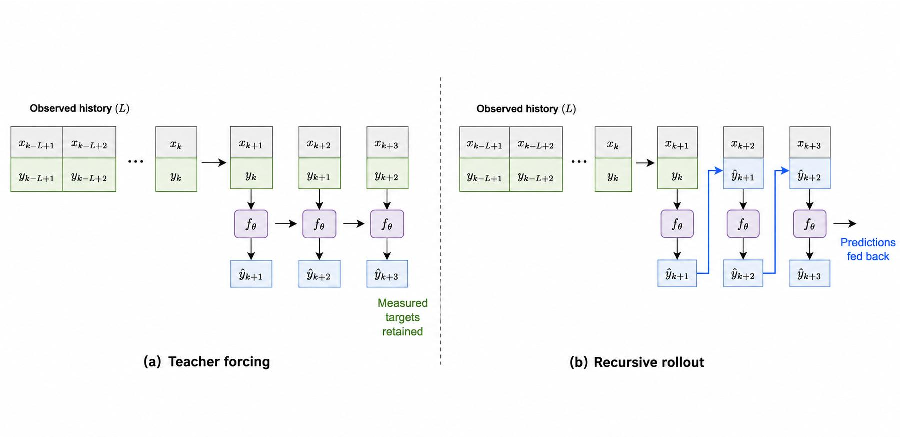
\includegraphics[width=\linewidth]
        {figures/fig_rollout_protocol.pdf}
        \caption{Teacher-forced and recursive rollout evaluation. Under teacher forcing, measured target history is supplied at successive prediction steps. Under recursive rollout, measured future targets are withheld after the initial history window and each predicted capacity--resistance pair is fed back into the subsequent input sequence.}
        \label{fig:rollout_protocol}
    \end{figure}
}{}

The sequence length $L$ and rollout horizon $H$ were treated as hyperparameters rather than fixed design choices. The search considered

\begin{equation}
L \in \{10,15,20\},
\end{equation}

and

\begin{equation}
H \in \{3,5,8,10,15\}.
\end{equation}

The longest eligible training trajectory contained 29 observations. A candidate was therefore considered feasible only when

\begin{equation}
L+H \leq 29.
\label{eq:trajectory_constraint}
\end{equation}

This coupled constraint is important because a rollout-training segment requires both the initial $L$-observation history and the subsequent $H$ prediction steps to exist within the same cell trajectory. An earlier manual setting of $L=20$ and $H=10$ violated this condition and consequently produced no valid rollout-training segments. The corrected manual reference uses $L=20$ and $H=8$.

Direct comparison of different sequence lengths introduces another issue. A model with $L=10$ can begin producing forecasts earlier in a trajectory than a model with $L=20$, so evaluating every configuration from its earliest possible prediction would give different models different scoring sets. A common evaluation window was therefore imposed across all candidate sequence lengths. Scoring begins at trajectory row index 20 for every configuration, corresponding to the largest candidate sequence length. Consequently, all optimisation methods and all sequence-length choices are compared on exactly the same observations.

After application of this common-window rule, the validation set contains 63 rollout evaluation points and the held-out test set contains 76 evaluation points. Hyperparameter optimisation and early stopping use only the common validation window. The 76-point held-out window remains untouched until the final configurations have been selected. This common-window design prevents an apparent optimiser advantage from arising simply because one sequence length was evaluated on an easier or shorter portion of the degradation trajectories.


% =========================================================
% 2.6 EVALUATION METRICS
% =========================================================

\subsection{Evaluation Metrics}
\label{sec:evaluation_metrics}

Prediction performance was evaluated after transforming the network outputs back to their original physical units. Capacity errors were therefore computed in ampere-hours and electrolyte-resistance errors in m$\Omega$, while percentage-based measures were evaluated from the corresponding unscaled target values.

For target $j \in \{Q,R_e\}$, mean absolute percentage error (MAPE) was defined as

\begin{equation}
\mathrm{MAPE}_{j}
=
\frac{100}{N}
\sum_{i=1}^{N}
\left|
\frac{y_{i,j}-\hat{y}_{i,j}}
{y_{i,j}}
\right|,
\label{eq:mape}
\end{equation}

where $N$ is the number of evaluated observations, $y_{i,j}$ is the measured value, and $\hat{y}_{i,j}$ is the corresponding prediction. MAPE provides a dimensionless relative-error measure and is widely used for forecast assessment, although its behaviour becomes problematic when target values approach zero \cite{hyndman2006accuracy}. This limitation does not affect the present source-domain evaluation because both retained targets remain strictly separated from zero.

Since capacity and electrolyte resistance have different physical units and numerical scales, the principal predictive metric was the unweighted mean of their target-specific MAPEs,

\begin{equation}
\mathrm{MAPE}_{\mathrm{macro}}
=
\frac{1}{2}
\left(
\mathrm{MAPE}_{Q}
+
\mathrm{MAPE}_{R_e}
\right).
\label{eq:macro_mape}
\end{equation}

This macro aggregation gives the two degradation targets equal contribution to model selection and prevents the target with the larger numerical scale from dominating the optimisation criterion. The macro formulation in Eq.~\eqref{eq:macro_mape} is specific to the two-output forecasting problem considered here, whereas the underlying target-wise MAPE follows the conventional percentage-error definition \cite{hyndman2006accuracy}.

Root mean square error (RMSE) was retained as a complementary physical-unit error measure,

\begin{equation}
\mathrm{RMSE}_{j}
=
\sqrt{
\frac{1}{N}
\sum_{i=1}^{N}
\left(
y_{i,j}-\hat{y}_{i,j}
\right)^2
},
\label{eq:rmse}
\end{equation}

which places greater weight on larger residuals through the squared-error term. RMSE and absolute-error measures are commonly reported together because they characterize different aspects of the residual distribution \cite{willmott2005mae}.

The coefficient of determination was additionally calculated as

\begin{equation}
R_j^2
=
1-
\frac{
\sum_{i=1}^{N}
\left(
y_{i,j}-\hat{y}_{i,j}
\right)^2
}{
\sum_{i=1}^{N}
\left(
y_{i,j}-\bar{y}_{j}
\right)^2
},
\label{eq:r2}
\end{equation}

where $\bar{y}_{j}$ is the mean measured value of target $j$. The $R^2$ statistic complements absolute and percentage errors by evaluating predictive performance relative to a constant predictor based on the target mean \cite{chicco2021r2}. Values approaching one indicate close agreement with the observations, whereas $R^2<0$ indicates that the model performs worse than the corresponding mean-value predictor.

The external transfer analysis was evaluated for capacity only because the resistance quantities in the source and external datasets are obtained using different measurement procedures. Capacity MAPE, RMSE, and $R^2$ were therefore reported independently for the external-domain experiments rather than combined with a resistance error.

Model efficiency was represented by trainable parameter count and measured inference latency. Parameter count was obtained directly from the trainable tensors of each candidate network,

\begin{equation}
P(\boldsymbol{\theta})
=
\sum_{\ell=1}^{L_{\theta}}
\operatorname{numel}
\left(
\boldsymbol{\theta}_{\ell}
\right),
\label{eq:param_count}
\end{equation}

where $\boldsymbol{\theta}_{\ell}$ denotes a trainable parameter tensor. Parameter count and inference latency are established complementary complexity criteria in multi-objective neural architecture optimisation because a smaller parameter set does not necessarily imply proportionally faster execution on a given computational platform \cite{phan2024monas}.

The latency objective used during hyperparameter search was the median batch-one forward-pass latency of a single input window. Twenty untimed warm-up passes were executed before measurement, followed by five timed blocks, and the median recorded time was retained:

\begin{equation}
T_{\mathrm{search}}
=
\operatorname{median}
\left(
t_{1},t_{2},\ldots,t_{5}
\right).
\label{eq:search_latency}
\end{equation}

Directly measured latency was used rather than a proxy such as parameter count or floating-point operation count because architectural complexity and hardware execution time need not vary proportionally \cite{tan2019mnasnet}.

The search-stage latency in Eq.~\eqref{eq:search_latency} should not be confused with the full-trajectory latency reported for the final confirmed models. Search latency measures one batch-one forward pass and is used as an optimisation objective. Full-trajectory latency includes every recursive forward call required to forecast a complete held-out trajectory and is reported separately as a deployment-oriented runtime measure.


% =========================================================
% 3. PROPOSED MULTI-OBJECTIVE OPTIMISATION FRAMEWORK
% =========================================================

\section{Proposed Multi-Objective Optimisation Framework}
\label{sec:optimisation_framework}

The optimisation framework was used to search for recurrent forecasting configurations that balanced predictive accuracy, model complexity, and inference cost under the recursive evaluation protocol defined in Section~\ref{sec:recursive_formulation}. All candidate configurations used the same forecasting backbone and training procedure. The optimisation algorithms therefore differed only in how candidate hyperparameter configurations were generated and retained, allowing their search behaviour to be compared under matched computational conditions.

% =========================================================
% 3.1 CANDIDATE LSTM FORECASTING MODEL
% =========================================================

\subsection{Candidate LSTM Forecasting Model}
\label{sec:lstm_model}

The forecasting backbone was a stacked long short-term memory (LSTM) network \cite{hochreiter1997lstm}. LSTM was selected because the degradation records form ordered cell-specific trajectories and the recurrent state provides a direct mechanism for retaining information from preceding health observations. The architecture itself was kept deliberately compact so that the optimisation study focuses on the effect of sequence length, recurrent capacity, depth, rollout horizon, and learning rate rather than on a large number of architecture-specific design choices.

At each observation step, the recurrent input contained the nine exogenous variables defined in Eq.~\eqref{eq:input_vector} together with the capacity and electrolyte-resistance history channels. The resulting per-step input therefore contained 11 variables,

\begin{equation}
\mathbf{u}_{c,k}
=
\left[
\mathbf{x}_{c,k},
Q^{*}_{c,k-1},
R^{*}_{e,c,k-1}
\right]^{\mathrm{T}},
\label{eq:lstm_input}
\end{equation}

where the superscript $*$ indicates that the history value depends on the evaluation mode. During teacher-forced training, $Q^{*}$ and $R^{*}_{e}$ were measured values. During recursive rollout, they were replaced by the model's preceding predictions after the observed history window.

For a sequence of length $L$, the recurrent encoder produces hidden states

\begin{equation}
\mathbf{h}_{1:L}
=
\operatorname{LSTM}_{\boldsymbol{\theta}}
\left(
\mathbf{u}_{1:L}
\right).
\label{eq:lstm_encoder}
\end{equation}

Only the final recurrent state $\mathbf{h}_{L}$ is passed to the regression head. The prediction mapping is

\begin{align}
\mathbf{z}_{1}
&=
\operatorname{Dropout}_{0.1}
\left[
\operatorname{ReLU}
\left(
\mathbf{W}_{1}\mathbf{h}_{L}+\mathbf{b}_{1}
\right)
\right],
\\
\mathbf{z}_{2}
&=
\operatorname{ReLU}
\left(
\mathbf{W}_{2}\mathbf{z}_{1}+\mathbf{b}_{2}
\right),
\\
\hat{\mathbf{y}}
&=
\mathbf{W}_{3}\mathbf{z}_{2}+\mathbf{b}_{3},
\label{eq:lstm_head}
\end{align}

where the first dense layer maps the candidate-dependent recurrent hidden dimension to 128 units, the second maps 128 to 64 units, and the final linear layer produces the two scaled outputs $\hat{Q}$ and $\hat{R}_{e}$. A recurrent dropout rate of 0.2 was used when the LSTM contained more than one layer; no recurrent dropout was applied to a single-layer candidate.

Table~\ref{tab:lstm_architecture} separates the hyperparameters exposed to optimisation from the architectural components held fixed across all candidates.

\begin{table}[htbp]
\centering
\caption{Structure of the candidate LSTM forecasting model.}
\label{tab:lstm_architecture}
\begin{tabular}{lll}
\toprule
\textbf{Component} &
\textbf{Setting} &
\textbf{Status} \\
\midrule
Input channels &
9 exogenous + 2 target-history channels &
Fixed \\

Sequence length $L$ &
10, 15, or 20 &
Optimised \\

LSTM hidden width &
64, 96, 128, 160, or 192 &
Optimised \\

Number of LSTM layers &
1, 2, or 3 &
Optimised \\

LSTM dropout &
0.2 for depth $>1$; otherwise 0 &
Fixed rule \\

Dense layer 1 &
Hidden width $\rightarrow 128$, ReLU &
Fixed \\

Dropout &
0.1 &
Fixed \\

Dense layer 2 &
128 $\rightarrow 64$, ReLU &
Fixed \\

Output layer &
64 $\rightarrow 2$ &
Fixed \\

Rollout horizon $H$ &
3, 5, 8, 10, or 15 &
Optimised \\

Learning rate $\eta$ &
$10^{-4}$ to $2\times10^{-3}$ &
Optimised \\
\bottomrule
\end{tabular}
\end{table}

Training was performed in two stages. The first stage provided a stable supervised initialization using measured target history. The network parameters were optimized using AdamW \cite{loshchilov2019adamw} with candidate learning rate $\eta$, weight decay $10^{-5}$, batch size 512, and Smooth-L1 prediction loss in scaled target space. The gradient norm was clipped at 1.0. Validation macro MAPE governed early stopping, and the checkpoint with the lowest validation error was restored before rollout fine-tuning.

Let $\mathcal{B}$ denote a teacher-forced minibatch. The first-stage objective can be written as

\begin{equation}
\mathcal{L}_{\mathrm{TF}}
=
\frac{1}{|\mathcal{B}|}
\sum_{i\in\mathcal{B}}
\operatorname{SmoothL1}
\left(
\mathbf{y}_{i},
\hat{\mathbf{y}}_{i}
\right).
\label{eq:teacher_loss}
\end{equation}

The second stage adapted the network specifically to recursive prediction. Each rollout-training sample contained an initial window of $L$ observations followed by $H$ future exogenous observations and their corresponding targets. Successive training segments were generated with a stride of two observations. Starting from the measured initial history, the model predicts the first future target pair. That prediction is concatenated with the known exogenous variables at the next step and returned to the recurrent input. The process is repeated for all $H$ steps.

For a rollout beginning at index $k$, the recursive training objective is

\begin{equation}
\mathcal{L}_{\mathrm{RO}}
=
\frac{1}{H}
\sum_{s=1}^{H}
\left\|
\mathbf{y}_{c,k+s}
-
\hat{\mathbf{y}}_{c,k+s}
\right\|_{2}^{2}.
\label{eq:rollout_loss}
\end{equation}

The rollout stage used AdamW with learning rate $0.30\eta$, weight decay $10^{-5}$, batch size 128, and gradient-norm clipping at 1.0. Early stopping was based on common-window validation rollout macro MAPE rather than teacher-forced error, and the best rollout checkpoint is restored. This criterion kept the training objective aligned with the deployment-oriented evaluation used during optimisation.

The two-stage procedure was applied identically to every candidate generated by NSGA-II, NSGA-III, or random search. Candidate quality therefore reflected the selected hyperparameters and search strategy rather than differences in model architecture, optimiser family, loss construction, or validation protocol.

% =========================================================
% 3.2 MULTI-OBJECTIVE SEARCH PROBLEM AND SEARCH SPACE
% =========================================================

\subsection{Multi-Objective Search Problem and Search Space}
\label{sec:search_problem}

Hyperparameter selection was formulated as a constrained three-objective optimisation problem. Each candidate configuration specified the temporal context available to the recurrent model, its representational capacity, the depth of the recurrent stack, the rollout horizon used during recursive fine-tuning, and the learning rate. The objective was not to identify a single configuration with minimum prediction error, but to obtain a set of nondominated configurations representing different compromises between predictive accuracy, model size, and inference cost.

A candidate configuration was represented as

\begin{equation}
\boldsymbol{\omega}
=
\left[
L,\,
d_h,\,
n_{\mathrm{LSTM}},\,
H,\,
\eta
\right],
\label{eq:candidate_vector}
\end{equation}

where $L$ is the input sequence length, $d_h$ is the LSTM hidden width, $n_{\mathrm{LSTM}}$ is the number of recurrent layers, $H$ is the recursive rollout horizon, and $\eta$ is the initial learning rate. The corresponding search domains were

\begin{align}
L &\in \{10,15,20\}, \\
d_h &\in \{64,96,128,160,192\}, \\
n_{\mathrm{LSTM}} &\in \{1,2,3\}, \\
H &\in \{3,5,8,10,15\}, \\
\eta &\in [10^{-4},\,2\times10^{-3}],
\label{eq:search_domains}
\end{align}

with $\eta$ sampled and mutated on a logarithmic scale. The resulting search space is mixed discrete--continuous and includes the coupled feasibility constraint

\begin{equation}
L+H\leq29,
\label{eq:search_feasibility}
\end{equation}

which follows from the length of the longest sequence available for rollout training. Candidate configurations violating Eq.~\eqref{eq:search_feasibility} are repaired during evolutionary search rather than discarded.

The three optimisation objectives were all minimised. For candidate $\boldsymbol{\omega}$, the objective vector was defined as

\begin{equation}
\mathbf{F}(\boldsymbol{\omega})
=
\left[
f_{1}(\boldsymbol{\omega}),
f_{2}(\boldsymbol{\omega}),
f_{3}(\boldsymbol{\omega})
\right]^{\mathrm{T}},
\label{eq:objective_vector}
\end{equation}

where

\begin{align}
f_{1}(\boldsymbol{\omega})
&=
\mathrm{MAPE}_{\mathrm{macro,val}}^{\mathrm{rollout}},
\label{eq:objective_mape}
\\
f_{2}(\boldsymbol{\omega})
&=
P(\boldsymbol{\omega}),
\label{eq:objective_parameters}
\\
f_{3}(\boldsymbol{\omega})
&=
T_{\mathrm{search}}(\boldsymbol{\omega}).
\label{eq:objective_latency}
\end{align}

The first objective was the common-window validation macro MAPE obtained under recursive rollout. It therefore evaluates a candidate using the same deployment-oriented prediction setting used for final model assessment. The second objective was the number of trainable parameters defined in Eq.~\eqref{eq:param_count}. The third objective was the median batch-one forward-pass latency defined in Eq.~\eqref{eq:search_latency}. Model complexity and latency were retained as separate objectives because parameter count is hardware-independent, whereas observed execution time also depends on the computational structure of the network and the execution platform \cite{tan2019mnasnet,phan2024monas}.

For two feasible candidates $\boldsymbol{\omega}^{(a)}$ and $\boldsymbol{\omega}^{(b)}$, candidate $a$ dominates candidate $b$ when

\begin{equation}
f_j\!\left(\boldsymbol{\omega}^{(a)}\right)
\leq
f_j\!\left(\boldsymbol{\omega}^{(b)}\right)
\quad
\forall j\in\{1,2,3\},
\end{equation}

and

\begin{equation}
f_j\!\left(\boldsymbol{\omega}^{(a)}\right)
<
f_j\!\left(\boldsymbol{\omega}^{(b)}\right)
\quad
\text{for at least one }j.
\label{eq:pareto_dominance}
\end{equation}

The nondominated candidates formed an approximation to the Pareto front. This formulation avoided assigning fixed scalar weights to prediction error, parameter count, and latency before optimisation. NSGA-II and NSGA-III are specifically designed to retain such nondominated trade-offs during population-based search \cite{deb2002nsga2,deb2014nsga3}.

Random search was retained as a matched-budget non-evolutionary reference. It samples the same discrete domains and the same log-uniform learning-rate interval, applies the same feasibility condition, and evaluates candidates through the identical training and validation pipeline. Random search is a relevant baseline for hyperparameter optimisation because it does not impose a population-selection mechanism and can remain competitive when only a subset of the available hyperparameters strongly influences model performance \cite{bergstra2012random}. Consequently, differences between the three search methods can be attributed to candidate-generation and selection behaviour rather than to differences in search space, model training, or objective computation.

\IfFileExists{figures/fig_optimisation_framework.pdf}{
    The complete optimisation process is summarised in Figure~\ref{fig:optimisation_framework}.

    \begin{figure}[htbp]
        \centering
        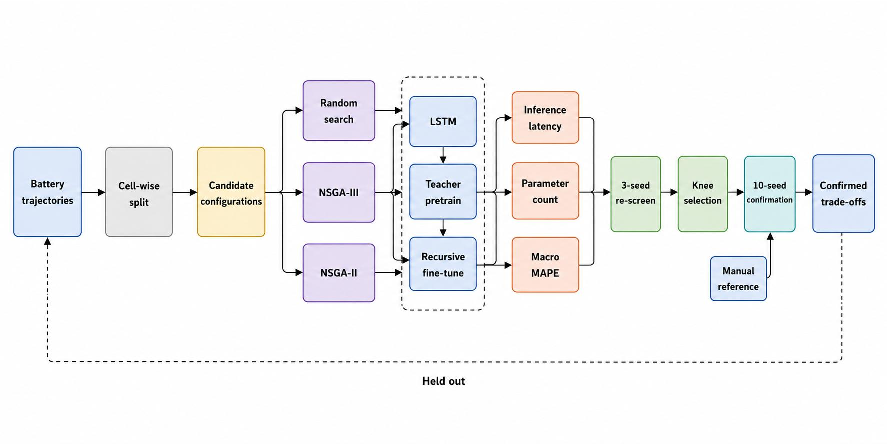
\includegraphics[width=\linewidth]
        {figures/fig_optimisation_framework.pdf}
        \caption{Multi-objective hyperparameter optimisation framework. Candidate LSTM configurations are generated within the constrained mixed search space, trained using the common two-stage forecasting procedure, and evaluated under recursive rollout using validation macro MAPE, trainable parameter count, and batch-one inference latency. NSGA-II, NSGA-III, and matched-budget random search operate on the same candidate representation and evaluation pipeline. Selected nondominated candidates subsequently undergo multi-seed re-screening and final confirmation.}
        \label{fig:optimisation_framework}
    \end{figure}
}{}

Table~\ref{tab:search_space} summarises the decision variables and their domains.

\begin{table}[htbp]
\centering
\caption{Hyperparameter search space used by NSGA-II, NSGA-III, and matched-budget random search.}
\label{tab:search_space}
\begin{tabular}{llll}
\toprule
\textbf{Variable} &
\textbf{Symbol} &
\textbf{Domain} &
\textbf{Type} \\
\midrule
Sequence length &
$L$ &
$\{10,15,20\}$ &
Discrete \\

Hidden width &
$d_h$ &
$\{64,96,128,160,192\}$ &
Discrete \\

LSTM layers &
$n_{\mathrm{LSTM}}$ &
$\{1,2,3\}$ &
Discrete \\

Rollout horizon &
$H$ &
$\{3,5,8,10,15\}$ &
Discrete \\

Learning rate &
$\eta$ &
$10^{-4}$--$2\times10^{-3}$ &
Log-continuous \\
\bottomrule
\end{tabular}

\vspace{2mm}
\footnotesize{\textit{Constraint:} $L+H\leq29$.}
\end{table}

% =========================================================
% 3.3 EVOLUTIONARY SEARCH PROCEDURES
% =========================================================

\subsection{Evolutionary Search Procedures}
\label{sec:evolutionary_search}

NSGA-II and NSGA-III were implemented over the same candidate representation, feasibility rule, variation operators, objective functions, and evaluation pipeline. Their comparison therefore isolates the effect of the environmental-selection mechanism: crowding-distance preservation in NSGA-II and reference-direction niching in NSGA-III \cite{deb2002nsga2,deb2014nsga3}. Both algorithms operate directly on the mixed discrete--continuous decision vector defined in Eq.~\eqref{eq:candidate_vector}.

% ---------------------------------------------------------
% 3.3.1 COMMON VARIATION OPERATORS
% ---------------------------------------------------------

\subsubsection{Common Variation Operators}
\label{sec:variation_operators}

Parent configurations were recombined using uniform per-variable crossover. For each decision variable, the offspring inherited the value from either parent with equal probability. If $\boldsymbol{\omega}^{(a)}$ and $\boldsymbol{\omega}^{(b)}$ denote two parent configurations, the $j$th offspring component was generated as

\begin{equation}
\omega^{(c)}_{j}
=
\begin{cases}
\omega^{(a)}_{j}, & r_j < 0.5,\\
\omega^{(b)}_{j}, & r_j \geq 0.5,
\end{cases}
\label{eq:uniform_crossover}
\end{equation}

where $r_j\sim\mathcal{U}(0,1)$ is sampled independently for each decision variable.

Mutation was subsequently applied independently to the four discrete variables $L$, $d_h$, $n_{\mathrm{LSTM}}$, and $H$, each with probability 0.25. A selected discrete variable was replaced by another admissible value from its corresponding domain.

The learning rate was mutated separately with probability 0.25. Because learning rates span multiplicative rather than additive scales, perturbation was performed in base-10 logarithmic space:

\begin{equation}
\log_{10}\eta'
=
\log_{10}\eta+\epsilon,
\qquad
\epsilon\sim\mathcal{N}(0,0.28^2),
\label{eq:lr_mutation}
\end{equation}

after which $\eta'$ was clipped to the interval

\begin{equation}
10^{-4}\leq\eta'\leq2\times10^{-3}.
\end{equation}

To ensure that every generated offspring differed from its inherited parent configuration, one randomly selected decision variable was forced to mutate whenever none of the variables had changed during the independent mutation step.

The coupled constraint between sequence length and rollout horizon was handled through repair rather than candidate rejection. For an offspring satisfying

\begin{equation}
L+H>29,
\end{equation}

the rollout horizon was replaced by the admissible value in

\begin{equation}
\mathcal{H}_{L}
=
\left\{
h\in\{3,5,8,10,15\}:L+h\leq29
\right\}
\end{equation}

that was closest to the originally generated value. When two feasible horizons were equally distant, the larger value was retained. This repair rule preserves the generated sequence-length choice while restoring the trajectory-length constraint in Eq.~\eqref{eq:search_feasibility}.

Duplicate configurations were not counted as new evaluations. When a generated offspring duplicated a configuration already evaluated within the same search run, a new candidate was generated until a previously unevaluated feasible configuration was obtained. Consequently, the computational budget refers to unique trained configurations rather than attempted offspring generation.

% ---------------------------------------------------------
% 3.3.2 NSGA-II
% ---------------------------------------------------------

\subsubsection{NSGA-II}
\label{sec:nsga2}

NSGA-II uses Pareto rank as the primary selection criterion and crowding distance to preserve diversity among solutions belonging to the same nondominated front \cite{deb2002nsga2}. Parent selection was performed by binary tournament. For two competing candidates, the candidate with the better Pareto rank was preferred; when both belonged to the same front, the candidate with the larger crowding distance was selected.

At each generation, the parent population $\mathcal{P}_{t}$ and offspring population $\mathcal{Q}_{t}$ were combined,

\begin{equation}
\mathcal{R}_{t}
=
\mathcal{P}_{t}\cup\mathcal{Q}_{t}.
\label{eq:nsga2_combined_population}
\end{equation}

Fast nondominated sorting partitioned $\mathcal{R}_{t}$ into fronts

\begin{equation}
\mathcal{F}_{1},
\mathcal{F}_{2},
\ldots,
\mathcal{F}_{m},
\end{equation}

ordered from the best nondominated rank to progressively dominated fronts. Complete fronts were transferred to the next population until addition of another complete front would exceed the prescribed population size. When the final admissible front could only be included partially, its candidates were ordered by decreasing crowding distance and the most widely separated solutions were retained. This procedure promotes convergence while maintaining coverage of the three-dimensional objective trade-off surface.

% ---------------------------------------------------------
% 3.3.3 NSGA-III
% ---------------------------------------------------------

\subsubsection{NSGA-III}
\label{sec:nsga3}

NSGA-III retains nondominated sorting but replaces crowding-distance truncation with reference-direction-based niching \cite{deb2014nsga3}. For the three-objective problem considered here, a Das--Dennis simplex construction with division parameter $p=6$ produced 28 reference directions,

\begin{equation}
N_{\mathrm{ref}}
=
\binom{M+p-1}{p}
=
\binom{3+6-1}{6}
=
28,
\label{eq:reference_direction_count}
\end{equation}

where $M=3$ is the number of objectives. The number of reference directions therefore matched the evolutionary population size exactly.

Because macro MAPE, parameter count, and latency occupy different numerical ranges, the three objectives were min--max normalised within the combined parent--offspring population before reference-direction association. For objective $j$,

\begin{equation}
\tilde{f}_{j}
=
\frac{
f_j-f_{j,\min}
}{
f_{j,\max}-f_{j,\min}
},
\label{eq:nsga3_normalisation}
\end{equation}

where the extrema were calculated from the combined population at the current generation.

Each candidate was associated with the reference direction having the smallest perpendicular distance from its normalised objective vector. As in NSGA-II, complete nondominated fronts were first transferred directly to the next population. When only part of the final front could be retained, candidates were selected through reference-direction niching. Reference niches with the smallest current occupancy were considered first. For an unoccupied niche, the associated candidate with the smallest perpendicular distance to that reference direction was selected. If the niche was already occupied, one of its remaining associated candidates was selected randomly. The process continued until the population was filled.

The use of 28 fixed reference directions provides an explicit diversity structure for NSGA-III, whereas NSGA-II relies on local crowding distance. No algorithm-specific change was made to the candidate representation, neural-network training schedule, objective computation, feasibility repair, or unique-evaluation rule. The resulting comparison therefore examines whether the two diversity-preservation mechanisms differ in their ability to discover useful error--complexity--latency trade-offs.

Table~\ref{tab:evolutionary_comparison} summarises the elements shared by the two evolutionary methods and the selection mechanism that distinguishes them.

\begin{table}[htbp]
\centering
\caption{Common and algorithm-specific components of NSGA-II and NSGA-III.}
\label{tab:evolutionary_comparison}
\begin{tabular}{lll}
\toprule
\textbf{Component} &
\textbf{NSGA-II} &
\textbf{NSGA-III} \\
\midrule
Objectives &
3, all minimised &
3, all minimised \\

Population size &
28 &
28 \\

Parent--offspring combination &
Yes &
Yes \\

Nondominated sorting &
Yes &
Yes \\

Crossover &
Uniform per variable &
Uniform per variable \\

Discrete mutation probability &
0.25 per variable &
0.25 per variable \\

Learning-rate mutation &
Log-space Gaussian &
Log-space Gaussian \\

Constraint handling &
Feasibility repair &
Feasibility repair \\

Duplicate handling &
Regeneration &
Regeneration \\

Diversity mechanism &
Crowding distance &
Reference-direction niching \\

Reference directions &
-- &
28 ($p=6$) \\

Split-front selection &
Largest crowding distance &
Least-occupied reference niches \\
\bottomrule
\end{tabular}
\end{table}


% =========================================================
% 3.4 MATCHED-BUDGET RANDOM SEARCH
% =========================================================

\subsection{Matched-Budget Random Search}
\label{sec:random_search}

Random search was included as a non-evolutionary reference for determining whether the population-based search mechanisms of NSGA-II and NSGA-III provide an advantage beyond direct sampling of the same hyperparameter space. Random search is an appropriate baseline for hyperparameter optimisation because it does not allocate trials systematically along every search dimension and can remain competitive when model performance depends strongly on only a subset of the available hyperparameters \cite{bergstra2012random}.

Each random-search candidate was drawn from the same mixed discrete--continuous domain defined in Eq.~\eqref{eq:search_domains}. The four discrete variables were sampled uniformly from their respective admissible sets,

\begin{align}
L &\sim \mathcal{U}\{10,15,20\},\\
d_h &\sim \mathcal{U}\{64,96,128,160,192\},\\
n_{\mathrm{LSTM}} &\sim \mathcal{U}\{1,2,3\},\\
H &\sim \mathcal{U}\{3,5,8,10,15\},
\end{align}

subject to the feasibility condition

\begin{equation}
L+H\leq29.
\end{equation}

The learning rate was sampled uniformly in logarithmic rather than linear space,

\begin{equation}
\log_{10}\eta
\sim
\mathcal{U}
\left(
\log_{10}10^{-4},
\log_{10}(2\times10^{-3})
\right),
\label{eq:random_lr}
\end{equation}

which gives comparable sampling opportunity across multiplicative learning-rate scales.

Every accepted configuration was unique within its search run. A configuration that had already been evaluated in the same run was regenerated and did not consume the unique-evaluation budget. Each retained candidate was trained using the same two-stage LSTM procedure described in Section~\ref{sec:lstm_model} and was evaluated using the same three objectives,

\begin{equation}
\mathbf{F}(\boldsymbol{\omega})
=
\left[
\mathrm{MAPE}_{\mathrm{macro,val}}^{\mathrm{rollout}},
P(\boldsymbol{\omega}),
T_{\mathrm{search}}(\boldsymbol{\omega})
\right]^{\mathrm{T}}.
\end{equation}

Unlike NSGA-II and NSGA-III, random search does not use objective values from previously evaluated candidates to determine which configuration should be generated next. It therefore contains no parent selection, crossover, mutation, nondominated survival, crowding-distance calculation, or reference-direction niching. Its role was to measure the trade-off quality obtainable from the same search domain and computational budget without evolutionary guidance.

The comparison was otherwise fully matched. Random search used the same feasible search space, candidate-training schedule, objective definitions, latency measurement procedure, run-wise training seeds, and number of unique model evaluations as the two evolutionary methods. The exact evaluation budget and run-wise seed pairing are specified in Section~\ref{sec:experimental_design}. This design ensures that subsequent differences in Pareto-front quality and convergence cannot be attributed to unequal model-training budgets or different candidate-evaluation procedures.


% =========================================================
% 3.5 PARETO-FRONT QUALITY AND CONVERGENCE INDICATORS
% =========================================================

\subsection{Pareto-Front Quality and Convergence Indicators}
\label{sec:pareto_indicators}

The outcome of a multi-objective search is an approximation set rather than a single optimum. Evaluating only the candidate with the smallest prediction error would therefore ignore whether an optimiser discovers useful trade-offs between predictive accuracy, model size, and inference latency. The three search methods were consequently compared using hypervolume (HV), inverted generational distance (IGD), IGD$^{+}$, and Schott spacing. These indicators quantify complementary properties of approximation-set quality, including convergence toward the best-known trade-off surface, objective-space coverage, and local distribution of nondominated solutions \cite{zitzler2003performance,ishibuchi2019indicators,schott1995spacing}.

\subsubsection{Global Objective Transformation and Normalisation}
\label{sec:indicator_normalisation}

Indicator values are sensitive to differences in objective scale. This is particularly relevant here because macro MAPE is expressed as a percentage, parameter count spans orders of magnitude, and latency is measured in milliseconds. Indicator computation was therefore performed in a common transformed and globally normalised objective space.

All 12,600 candidate evaluations from NSGA-II, NSGA-III, and random search were pooled before indicator calculation. Each raw objective vector was first transformed as

\begin{equation}
\mathbf{g}(\boldsymbol{\omega})
=
\left[
f_1(\boldsymbol{\omega}),
\log_{10} f_2(\boldsymbol{\omega}),
\log_{10} f_3(\boldsymbol{\omega})
\right]^{\mathrm{T}},
\label{eq:indicator_transform}
\end{equation}

where $f_1$ is validation rollout macro MAPE, $f_2$ is trainable parameter count, and $f_3$ is measured inference latency. Logarithmic transformation was applied to the two resource objectives because both vary multiplicatively across the search space.

The global lower and upper bounds observed across the complete 12,600-evaluation pool were

\begin{equation}
\mathbf{g}_{\min}
=
\begin{bmatrix}
0.7308796223\\
4.5613160916\\
-0.4342352697
\end{bmatrix},
\qquad
\mathbf{g}_{\max}
=
\begin{bmatrix}
8.8913714513\\
5.8939979806\\
0.0246944637
\end{bmatrix}.
\label{eq:indicator_bounds}
\end{equation}

Each transformed objective was then mapped to the interval $[0,1]$ using

\begin{equation}
z_j
=
\frac{
g_j-g_{j,\min}
}{
g_{j,\max}-g_{j,\min}
},
\qquad j=1,2,3.
\label{eq:indicator_normalisation}
\end{equation}

The same fixed global bounds were used for every optimiser, every independent run, and every convergence checkpoint. This avoids changing the geometry of the objective space from one method or evaluation budget to another.

% ---------------------------------------------------------
% HYPERVOLUME
% ---------------------------------------------------------

\subsubsection{Hypervolume}
\label{sec:hypervolume_metric}

Hypervolume measures the portion of objective space weakly dominated by an approximation set and bounded by a prescribed reference point \cite{zitzler2003performance,ishibuchi2019indicators}. For a nondominated approximation set $\mathcal{A}$ in the normalised minimisation space, HV was calculated as

\begin{equation}
\mathrm{HV}(\mathcal{A})
=
\lambda
\left(
\bigcup_{\mathbf{a}\in\mathcal{A}}
[\mathbf{a},\mathbf{r}_{\mathrm{HV}}]
\right),
\label{eq:hypervolume}
\end{equation}

where $\lambda(\cdot)$ denotes the three-dimensional Lebesgue measure and the fixed reference point was

\begin{equation}
\mathbf{r}_{\mathrm{HV}}
=
(1.1,\,1.1,\,1.1).
\label{eq:hv_reference}
\end{equation}

The reference point lies outside the globally normalised objective cube and was held constant for all comparisons. Larger HV indicates a more favourable combination of convergence and objective-space coverage.

% ---------------------------------------------------------
% IGD
% ---------------------------------------------------------

\subsubsection{Inverted Generational Distance}
\label{sec:igd_metric}

IGD measures the average distance from a reference approximation of the Pareto front to the closest solution returned by a search method \cite{ishibuchi2019indicators}. Because the true Pareto front is unknown for the present neural hyperparameter problem, a best-known empirical reference set was constructed from the pooled evaluations.

Let

\begin{equation}
\mathcal{R}
=
\operatorname{ND}
\left(
\mathcal{E}_{\mathrm{NSGA-II}}
\cup
\mathcal{E}_{\mathrm{NSGA-III}}
\cup
\mathcal{E}_{\mathrm{RS}}
\right)
\label{eq:igd_reference_set}
\end{equation}

denote the nondominated union of all 12,600 evaluated configurations after transformation and global normalisation. The resulting pooled reference set contained 28 nondominated points.

For approximation set $\mathcal{A}$, IGD was defined as

\begin{equation}
\mathrm{IGD}(\mathcal{A},\mathcal{R})
=
\frac{1}{|\mathcal{R}|}
\sum_{\mathbf{r}\in\mathcal{R}}
\min_{\mathbf{a}\in\mathcal{A}}
\left\|
\mathbf{r}-\mathbf{a}
\right\|_{2}.
\label{eq:igd}
\end{equation}

Smaller IGD indicates that the approximation set lies closer, on average, to the pooled best-known trade-off surface.

% ---------------------------------------------------------
% IGD+
% ---------------------------------------------------------

\subsubsection{IGD$^{+}$}
\label{sec:igdplus_metric}

Standard IGD is not Pareto compliant and can under some geometries favour a dominated approximation set. IGD$^{+}$ modifies the point-to-set distance so that only objective-wise deterioration relative to a reference solution contributes to the distance \cite{ishibuchi2019indicators}. For candidate point $\mathbf{a}$ and reference point $\mathbf{r}$, the modified distance was

\begin{equation}
d^{+}(\mathbf{r},\mathbf{a})
=
\sqrt{
\sum_{j=1}^{3}
\left[
\max
\left(
a_j-r_j,0
\right)
\right]^2
}.
\label{eq:igdplus_distance}
\end{equation}

IGD$^{+}$ was then calculated as

\begin{equation}
\mathrm{IGD}^{+}(\mathcal{A},\mathcal{R})
=
\frac{1}{|\mathcal{R}|}
\sum_{\mathbf{r}\in\mathcal{R}}
\min_{\mathbf{a}\in\mathcal{A}}
d^{+}(\mathbf{r},\mathbf{a}).
\label{eq:igdplus}
\end{equation}

As with IGD, smaller values are preferred. IGD$^{+}$ was retained as a robustness check because its dominance-aware distance provides a complementary assessment to conventional IGD \cite{ishibuchi2019indicators}.

% ---------------------------------------------------------
% LEAVE-ONE-METHOD-OUT IGD
% ---------------------------------------------------------

\subsubsection{Leave-One-Method-Out IGD}
\label{sec:loo_igd}

The pooled IGD reference set in Eq.~\eqref{eq:igd_reference_set} necessarily contains solutions contributed by the methods being evaluated. A method that contributes many points to the pooled nondominated set could therefore be suspected of receiving an advantage from the reference-set construction itself. A leave-one-method-out IGD (LOO-IGD) analysis was introduced to test this possibility.

For a method $m$, the alternative reference set was reconstructed using only evaluations produced by the other two search methods,

\begin{equation}
\mathcal{R}_{-m}
=
\operatorname{ND}
\left(
\bigcup_{q\neq m}
\mathcal{E}_{q}
\right).
\label{eq:loo_reference}
\end{equation}

The resulting method-excluded reference set contained 46 points for each leave-one-method-out comparison. LOO-IGD was then evaluated using the conventional IGD expression,

\begin{equation}
\mathrm{LOO\mbox{-}IGD}_{m}
=
\frac{1}{|\mathcal{R}_{-m}|}
\sum_{\mathbf{r}\in\mathcal{R}_{-m}}
\min_{\mathbf{a}\in\mathcal{A}_{m}}
\left\|
\mathbf{r}-\mathbf{a}
\right\|_{2}.
\label{eq:loo_igd}
\end{equation}

This analysis is not treated as a separate optimisation objective. It is a sensitivity test designed specifically to determine whether the ranking obtained with pooled-reference IGD persists when the scored method is prevented from contributing to its own reference set.

% ---------------------------------------------------------
% SCHOTT SPACING
% ---------------------------------------------------------

\subsubsection{Front Cardinality and Schott Spacing}
\label{sec:spacing_metric}

The number of nondominated solutions was recorded as a simple measure of approximation-set cardinality. Diversity within each nondominated set was additionally assessed using the spacing metric proposed by Schott \cite{schott1995spacing}.

For each point $\mathbf{a}_i$ in a nondominated set of size $n$, the distance to its nearest neighbouring solution was calculated in the globally normalised objective space as

\begin{equation}
d_i
=
\min_{\substack{k=1,\ldots,n\\k\neq i}}
\sum_{j=1}^{3}
\left|
a_{i,j}-a_{k,j}
\right|.
\label{eq:schott_distance}
\end{equation}

Let

\begin{equation}
\bar{d}
=
\frac{1}{n}
\sum_{i=1}^{n}d_i.
\end{equation}

Schott spacing was then calculated as

\begin{equation}
S
=
\sqrt{
\frac{1}{n-1}
\sum_{i=1}^{n}
\left(
d_i-\bar{d}
\right)^2
}.
\label{eq:schott_spacing}
\end{equation}

Smaller values indicate more even local spacing among the nondominated solutions. Spacing and front cardinality were analysed separately from HV and IGD because an optimiser may converge closer to the best-known Pareto front without producing a larger or more uniformly distributed approximation set.

% ---------------------------------------------------------
% CONVERGENCE CHECKPOINTS
% ---------------------------------------------------------

\subsubsection{Convergence Assessment}
\label{sec:indicator_convergence}

Indicator values were recomputed after every 28 unique candidate evaluations,

\begin{equation}
e
\in
\{28,56,84,\ldots,280\},
\label{eq:indicator_checkpoints}
\end{equation}

giving ten common budget checkpoints per independent search run. At each checkpoint, the nondominated approximation set formed from all candidates evaluated up to that budget was extracted and scored using the same global transformation, normalisation bounds, and indicator definitions.

Comparisons were therefore made against the number of completed neural-network evaluations rather than generation number. This is particularly important for the comparison with random search, which has no generation-based population update. Evaluation count provides a common computational axis for all three search methods and permits direct assessment of how rapidly each method approaches a given front-quality level.


% =========================================================
% 3.6 CANDIDATE RE-SCREENING AND FINAL CONFIGURATION SELECTION
% =========================================================

\subsection{Candidate Re-screening and Final Configuration Selection}
\label{sec:final_selection}

The configuration returned by a single search evaluation was not treated as final evidence because neural-network training introduces seed-dependent variation in prediction error and latency. A three-stage procedure was therefore used: multi-objective search, three-seed re-screening, and ten-seed final confirmation. The same procedure was applied to NSGA-II, NSGA-III, and random search.

For each search method, all nondominated configurations obtained across the 15 independent runs were first pooled. Candidate solutions were ordered by their normalised distance from the ideal objective vector, and the five highest-ranked unique configurations were retained. This produced a common re-screening set of 15 candidate configurations across the three search methods.

Each retained configuration was then retrained independently using seeds

\begin{equation}
\mathcal{S}_{\mathrm{re}}
=
\{42,52,62\}.
\label{eq:rescreen_seeds}
\end{equation}

For candidate $i$, the re-screened predictive score was the mean recursive validation macro MAPE across the three seeds,

\begin{equation}
\bar{E}_{i}
=
\frac{1}{3}
\sum_{s\in\mathcal{S}_{\mathrm{re}}}
E_{i,s},
\label{eq:rescreen_mape}
\end{equation}

where $E_{i,s}$ denotes the common-window rollout macro MAPE obtained for seed $s$. Parameter count remained deterministic for a given architecture, while latency was remeasured during the re-screening stage.

The three decision quantities used for finalist selection were

\begin{equation}
\mathbf{v}_{i}
=
\left[
\bar{E}_{i},
\log_{10}P_i,
\log_{10}\bar{T}_{i}
\right]^{\mathrm{T}},
\label{eq:rescreen_vector}
\end{equation}

where $P_i$ is trainable parameter count and $\bar{T}_{i}$ is the mean measured forward latency across the re-screening runs. Prediction error, log-parameter count, and log-latency were min--max normalised across all 15 re-screened candidates,

\begin{equation}
\tilde{v}_{i,j}
=
\frac{
v_{i,j}-v_{j,\min}
}{
v_{j,\max}-v_{j,\min}
},
\qquad
j\in\{1,2,3\}.
\label{eq:rescreen_normalisation}
\end{equation}

The normalised ideal point is therefore

\begin{equation}
\mathbf{v}^{*}=(0,0,0).
\end{equation}

A resource-aware knee score was calculated as the Euclidean distance from this ideal point,

\begin{equation}
D_i
=
\left\|
\tilde{\mathbf{v}}_i-\mathbf{v}^{*}
\right\|_2
=
\sqrt{
\tilde{v}_{i,1}^{\,2}
+
\tilde{v}_{i,2}^{\,2}
+
\tilde{v}_{i,3}^{\,2}
}.
\label{eq:knee_distance}
\end{equation}

Within each search method, the candidate with the smallest $D_i$ was selected as the finalist. The rule gives equal geometric weight to re-screened prediction error, logarithmic parameter count, and logarithmic latency after normalisation. It is therefore not an accuracy-priority rule. A configuration with slightly larger MAPE can be preferred when the reduction in model size or latency gives a better overall three-objective compromise. This choice was fixed before final ten-seed evaluation so that the final configuration was not selected retrospectively from held-out test performance.

The selected NSGA-II, NSGA-III, and random-search configurations were then compared with the corrected manually tuned reference configuration. Each of the four models was retrained using ten matched seeds,

\begin{equation}
\mathcal{S}_{\mathrm{final}}
=
\{42,52,62,72,82,92,102,112,122,132\}.
\label{eq:final_seeds}
\end{equation}

All four configurations were evaluated on the same 76-point held-out panel comprising ten cells. The final comparison therefore contained 40 independent model trainings. The ten-seed stage was used only for confirmation of configurations selected before test evaluation; it was not used to modify hyperparameters or to return candidates to the search process.

Table~\ref{tab:selection_pipeline} summarises the three stages.

\begin{table}[htbp]
\centering
\caption{Search, re-screening, and final-confirmation procedure.}
\label{tab:selection_pipeline}
\begin{tabular}{llll}
\toprule
\textbf{Stage} &
\textbf{Candidates} &
\textbf{Seeds} &
\textbf{Purpose} \\
\midrule
Search &
280 evaluations per run &
Run-specific &
Pareto-front discovery \\

Re-screening &
5 per method; 15 total &
42, 52, 62 &
Reduce single-training-seed dependence \\

Final confirmation &
Manual + 3 finalists &
42--132 in steps of 10 &
Matched ten-seed comparison \\
\bottomrule
\end{tabular}
\end{table}


% =========================================================
% 4. EXPERIMENTAL DESIGN
% =========================================================

\section{Experimental Design}
\label{sec:experimental_design}

% =========================================================
% 4.1 SEARCH BUDGET, INDEPENDENT RUNS, AND SEED PAIRING
% =========================================================

\subsection{Search Budget, Independent Runs, and Seed Pairing}
\label{sec:search_budget}

Stochastic optimisation algorithms cannot be compared reliably from a single execution because the observed outcome depends on the particular random realisation of the search. Independent repeated runs and statistical comparison of the resulting performance distributions were therefore used throughout the optimiser study \cite{derrac2011nonparam,latorre2021guidelines}.

NSGA-II, NSGA-III, and random search were each executed independently 15 times. Every run was allocated exactly 280 unique candidate evaluations. The resulting search programme contained 4,200 complete candidate evaluations per search method and 12,600 evaluations across the three methods. Each candidate evaluation comprised a complete neural-network training procedure, including teacher-forced pretraining, recursive rollout fine-tuning, validation rollout evaluation, parameter counting, and latency measurement. The computational budget therefore represents trained forecasting models rather than inexpensive analytical fitness-function evaluations.

For the evolutionary methods, the population size was 28. Ten successive evaluation blocks, including the initial population, were used, giving 280 candidate evaluations per run. The same evaluation counts,

\begin{equation}
e\in\{28,56,84,\ldots,280\},
\end{equation}

were used as common convergence checkpoints for random search. Comparison against the number of completed candidate evaluations rather than generation number gives all three methods the same computational axis.

Run-level random-number-generator seeds were

\begin{equation}
20270001,20270002,\ldots,20270015.
\label{eq:search_rng_seeds}
\end{equation}

The same run seed was assigned to the corresponding NSGA-II, NSGA-III, and random-search executions. Neural-network training seeds were independently defined as

\begin{equation}
41001,41002,\ldots,41015,
\label{eq:candidate_training_seeds}
\end{equation}

and were likewise paired by run index across the three search methods. Thus, run $r$ of each search method used the same prescribed search-level and candidate-training seed pair. This pairing reduces avoidable between-method variation and makes the repeated comparison more sensitive to differences in search behaviour.

The archived integrity checks confirmed that every method--run combination contained exactly 280 unique feasible evaluations, with no missing objective values, duplicate run/evaluation identifiers, or candidates violating the constraint $L+H\leq29$. The 28-candidate initial populations were also recorded for every run before method-specific search updates were applied.

Fifteen independent runs were selected as a compromise between repeated-run inference and neural-training cost. This is smaller than the larger run counts often used when benchmark fitness evaluations are inexpensive, but each evaluation in the present study requires complete recurrent-network training and rollout assessment. The 12,600 search evaluations alone accumulated approximately 18.78~h of recorded model-training time on the study hardware. Including the separate noise-floor, re-screening, and final-confirmation experiments, the complete optimisation programme accumulated 19.06~h of recorded model-training time. These quantities refer to logged model-training time and should not be interpreted as complete end-to-end wall-clock or GPU-hour measurements.

Table~\ref{tab:search_budget} summarises the matched experimental budget and seed design.

\begin{table}[htbp]
\centering
\caption{Matched search budget and repeated-run design used for optimiser comparison.}
\label{tab:search_budget}
\begin{tabular}{ll}
\toprule
\textbf{Setting} & \textbf{Value} \\
\midrule
Search methods &
NSGA-II, NSGA-III, random search \\

Independent runs per method &
15 \\

Population/reference size &
28 \\

Evaluation blocks per run &
10 \\

Unique evaluations per run &
280 \\

Evaluations per method &
4,200 \\

Total search evaluations &
12,600 \\

Run RNG seeds &
20270001--20270015 \\

Candidate-training seeds &
41001--41015 \\

Seed matching &
Paired by run index across methods \\

Convergence checkpoints &
28, 56, \ldots, 280 evaluations \\

Search-only recorded model-training time &
18.78~h \\

Full optimisation-programme recorded training time &
19.06~h \\
\bottomrule
\end{tabular}
\end{table}

% =========================================================
% 4.2 TRAINING SCHEDULES AND COMPUTATIONAL ENVIRONMENT
% =========================================================

\subsection{Training Schedules and Computational Environment}
\label{sec:training_environment}

The same two-stage training procedure described in Section~\ref{sec:lstm_model} was retained throughout hyperparameter search, candidate re-screening, and final confirmation. The stages differed only in the maximum number of training epochs and early-stopping patience. Shorter schedules were used during the large-scale search to control computational cost, while progressively longer schedules were used once the candidate set had been reduced.

Teacher-forced pretraining used AdamW \cite{loshchilov2019adamw} with the candidate-specific learning rate $\eta$, weight decay $10^{-5}$, batch size 512, and Smooth-L1 loss in scaled target space. Gradient norms were clipped at 1.0. Early stopping was governed by validation macro MAPE, and the checkpoint with the lowest validation error was restored before recursive fine-tuning.

Rollout fine-tuning used AdamW with learning rate

\begin{equation}
\eta_{\mathrm{RO}} = 0.30\eta,
\label{eq:rollout_learning_rate}
\end{equation}

weight decay $10^{-5}$, batch size 128, and the multi-step rollout loss defined in Eq.~\eqref{eq:rollout_loss}. Gradient norms were again clipped at 1.0. Early stopping was based exclusively on common-window validation rollout macro MAPE, and the best rollout checkpoint was restored before objective computation or held-out evaluation.

Table~\ref{tab:training_schedules} gives the schedules used at the three stages of the optimisation pipeline.

\begin{table}[htbp]
\centering
\caption{Training schedules used during search, candidate re-screening, and final confirmation.}
\label{tab:training_schedules}
\begin{tabular}{lrrrr}
\toprule
\textbf{Stage} &
\textbf{Teacher max.} &
\textbf{Teacher patience} &
\textbf{Rollout max.} &
\textbf{Rollout patience} \\
\midrule
Search &
80 &
18 &
15 &
5 \\

Re-screening &
160 &
30 &
30 &
10 \\

Final confirmation &
220 &
40 &
40 &
15 \\
\bottomrule
\end{tabular}
\end{table}

The search schedule was applied to all 12,600 candidate evaluations generated by NSGA-II, NSGA-III, and random search. Candidate re-screening used the longer intermediate schedule for the 15 retained configurations evaluated over three training seeds. The final schedule was applied only to the three optimiser-selected configurations and the manually specified reference model during ten-seed confirmation. Increasing the available training budget in this manner reduces the computational burden of broad exploration while allowing the final comparisons to use a more permissive convergence schedule.

All primary optimisation experiments were executed on a Kaggle environment equipped with a single NVIDIA Tesla T4 GPU. The software environment used Python 3.12.13 and PyTorch 2.10.0+cu128, with model training performed on CUDA. Python, NumPy, PyTorch CPU, and PyTorch CUDA random-number generators were explicitly seeded for each prescribed run. Shuffled data loaders were also supplied with seeded generators so that the run-level design described in Section~\ref{sec:search_budget} controlled the principal sources of stochasticity.

Search-stage inference latency was measured on the same Tesla T4 environment used for candidate training. For each trained candidate, 20 untimed batch-one forward passes were performed before five timed blocks, and the median observed value was retained as $T_{\mathrm{search}}$. All competing search methods therefore used latency values measured under the same hardware and software conditions. As stated in Section~\ref{sec:evaluation_metrics}, this single-window latency is an optimisation objective and is distinct from the complete recursive-trajectory latency reported for confirmed models.

The recorded model-training times for the three optimisation searches were 21,851.64~s for NSGA-II, 22,068.59~s for NSGA-III, and 23,705.43~s for random search. The corresponding accumulated training time for the 12,600 search evaluations was approximately 18.78~h.

When the separately recorded noise-floor experiment, candidate re-screening, and final-confirmation trainings are included, the complete optimisation programme contains 19.06~h of logged model-training time. These values describe accumulated recorded training time only. They are not reported as total end-to-end wall-clock time or GPU-hours because data loading, model serialization, inference benchmarking, result processing, and other pipeline operations were not enclosed by a common preserved timer.

Additional baseline and ablation experiments were executed in separate computational environments. Their runtime measurements are therefore not combined directly with the Tesla-T4 latency results. In particular, CPU-trained models are compared with the optimised LSTM models on predictive accuracy and hardware-independent quantities such as parameter count where appropriate, but not on a common runtime axis.

% =========================================================
% 4.3 TRAINING-NOISE CHARACTERISATION
% =========================================================

\subsection{Training-Noise Characterisation}
\label{sec:noise_protocol}

Neural-network training introduces stochastic variation even when the architecture, hyperparameters, data partition, and evaluation protocol are held fixed. This source of variation is particularly relevant in hyperparameter optimisation because small differences between candidate objective values may reflect training-seed effects rather than persistent differences between configurations. The magnitude of this variation was therefore measured explicitly before interpreting the repeated optimiser comparisons. This follows the broader recommendation that stochastic optimisation results should be assessed across repeated independent realizations rather than from isolated best runs \cite{derrac2011nonparam,latorre2021guidelines}.

The noise experiment used eight fixed LSTM configurations. Each configuration was trained independently using the ten seeds

\begin{equation}
\mathcal{S}_{\mathrm{noise}}
=
\{42,52,62,72,82,92,102,112,122,132\}.
\label{eq:noise_seeds}
\end{equation}

This produced 80 complete neural-network trainings. No architecture or hyperparameter was changed between seeds for a given configuration.

The eight configurations are listed in Table~\ref{tab:noise_configurations}. They were evaluated using the same teacher-pretraining and rollout-fine-tuning schedule used during the optimisation search, namely 80 maximum teacher-forced epochs with patience 18 followed by 15 maximum rollout epochs with patience 5.

\begin{table}[htbp]
\centering
\caption{Fixed configurations used to characterize training-seed variation.}
\label{tab:noise_configurations}
\small
\begin{tabular}{lrrrrr}
\toprule
\textbf{ID} &
\textbf{$L$} &
\textbf{$d_h$} &
\textbf{Layers} &
\textbf{$H$} &
\textbf{Learning rate} \\
\midrule
C1 & 10 & 128 & 2 & 15 & 0.00070000 \\
C2 & 10 & 192 & 3 & 10 & 0.00100000 \\
C3 & 10 & 64  & 1 & 3  & 0.00070000 \\
C4 & 15 & 64  & 2 & 10 & 0.00120000 \\
C5 & 15 & 96  & 1 & 5  & 0.00051649 \\
C6 & 20 & 160 & 3 & 5  & 0.00020000 \\
C7 & 20 & 192 & 2 & 8  & 0.00100000 \\
C8 & 20 & 96  & 1 & 3  & 0.00042092 \\
\bottomrule
\end{tabular}
\end{table}

For configuration $c$, the seed-wise recursive validation errors are denoted by

\begin{equation}
E_{c,s}
=
\mathrm{MAPE}^{\mathrm{rollout}}_{\mathrm{macro},c,s},
\end{equation}

where $s\in\mathcal{S}_{\mathrm{noise}}$. The mean error across the ten retrainings was calculated as

\begin{equation}
\bar{E}_{c}
=
\frac{1}{10}
\sum_{s\in\mathcal{S}_{\mathrm{noise}}}
E_{c,s},
\label{eq:noise_mean}
\end{equation}

and training-seed variability was quantified using the sample standard deviation,

\begin{equation}
s_{E,c}
=
\sqrt{
\frac{1}{9}
\sum_{s\in\mathcal{S}_{\mathrm{noise}}}
\left(
E_{c,s}-\bar{E}_{c}
\right)^2
}.
\label{eq:noise_sd}
\end{equation}

The same procedure was applied to the measured batch-one inference latency. If $T_{c,s}$ denotes the latency recorded for configuration $c$ under seed $s$, its across-seed standard deviation was calculated as

\begin{equation}
s_{T,c}
=
\sqrt{
\frac{1}{9}
\sum_{s\in\mathcal{S}_{\mathrm{noise}}}
\left(
T_{c,s}-\bar{T}_{c}
\right)^2
}.
\label{eq:latency_noise_sd}
\end{equation}

The purpose of this experiment was descriptive rather than model-selective. None of the eight configurations was promoted to the final comparison because of its noise-floor result, and the experiment did not alter the subsequent NSGA-II, NSGA-III, or random-search procedure. Instead, the measured distributions provided an empirical scale against which small search-stage accuracy differences could be interpreted and motivated the independent re-screening and ten-seed confirmation stages defined in Section~\ref{sec:final_selection}.

The resulting training-error and latency variability are reported at the beginning of Section~\ref{sec:results_discussion}, before the optimiser results are interpreted.

% =========================================================
% 4.4 STATISTICAL ANALYSIS
% =========================================================

\subsection{Statistical Analysis}
\label{sec:statistical_analysis}

Statistical analysis was designed around the experimental unit associated with each comparison. Independent optimisation runs were used for comparisons between search methods, matched training seeds were used for comparisons between confirmed forecasting configurations, and paired target cells were used for the external transfer analysis. All hypothesis tests were two-sided, with a significance level of $\alpha=0.05$. Non-parametric procedures were preferred because the number of repeated runs or seeds was modest and normality of the resulting performance distributions was not assumed \cite{derrac2011nonparam,latorre2021guidelines}.

% ---------------------------------------------------------
% OPTIMISER-LEVEL COMPARISONS
% ---------------------------------------------------------

For the optimiser comparison, hypervolume, IGD, IGD$^{+}$, leave-one-method-out IGD, front cardinality, and spacing were obtained independently from each of the 15 runs of NSGA-II, NSGA-III, and random search. For each indicator, equality across the three methods was first examined using the Kruskal--Wallis rank test \cite{kruskal1952ranks}. When the omnibus comparison was followed by pairwise analysis, two-sided Mann--Whitney $U$ tests were applied \cite{mann1947test}. The three pairwise $p$-values within an indicator family were adjusted using Holm's sequential procedure to control the family-wise error rate \cite{holm1979procedure}.

In addition to $p$-values, pairwise optimiser comparisons were accompanied by the Vargha--Delaney $A_{12}$ measure of stochastic superiority \cite{vargha2000critique}. For methods $A$ and $B$,

\begin{equation}
A_{12}
=
P(X_A>X_B)
+
\frac{1}{2}P(X_A=X_B),
\label{eq:a12}
\end{equation}

where $X_A$ and $X_B$ denote indicator values obtained from randomly selected independent runs of the two methods. A value of $A_{12}=0.5$ indicates no stochastic ordering, whereas values increasingly different from 0.5 indicate stronger separation between the two run distributions.

The direction of interpretation depends on the indicator. For hypervolume, larger values are preferable, so $A_{12}>0.5$ favours the first method. For IGD, IGD$^{+}$, leave-one-method-out IGD, and spacing, smaller values are preferable; consequently, $A_{12}<0.5$ favours the first method. Effect sizes were therefore interpreted together with the optimisation direction rather than by numerical magnitude alone.

% ---------------------------------------------------------
% FINALIST COMPARISONS
% ---------------------------------------------------------

The selected NSGA-II, NSGA-III, and random-search configurations were compared with the corrected manual reference using the ten matched training seeds defined in Eq.~\eqref{eq:final_seeds}. Because the same seed was used for each configuration within a comparison, seed-wise outcomes formed paired observations. Two-sided Wilcoxon signed-rank tests were therefore used for pairwise comparisons \cite{wilcoxon1945ranking}. Comparisons of the three optimiser-selected configurations against the manual reference were adjusted using Holm correction.

For configuration $m$, seed uncertainty was summarised using the sample mean and sample standard deviation,

\begin{equation}
s_m
=
\sqrt{
\frac{1}{n-1}
\sum_{i=1}^{n}
\left(
x_{m,i}-\bar{x}_{m}
\right)^2
},
\label{eq:seed_sd}
\end{equation}

with $n=10$ independently trained seeds. Ninety-five-percent confidence intervals for mean performance and paired mean differences were obtained using 10,000 bootstrap resamples \cite{efron1993bootstrap}. Bootstrap resampling was carried out over the seed-level observations rather than over individual prediction rows, preserving the trained model as the unit of replication.

Differences in seed-to-seed dispersion between the confirmed configurations were examined only as a secondary analysis. Levene and Brown--Forsythe tests were used to assess homogeneity of variance. Variance differences were not inferred from standard deviations alone.

% ---------------------------------------------------------
% GROUPED-FOLD COMPARISONS
% ---------------------------------------------------------

For the separate grouped five-fold model comparison, performance ranks were compared across the evaluated model variants using the Friedman test. The five held-out folds formed the repeated blocks. Because only five folds were available, pairwise exact Wilcoxon tests have a minimum attainable non-zero two-sided $p$-value of 0.0625. Pairwise superiority was therefore not inferred when the omnibus test rejected equality; model ranks and the omnibus result were reported without unsupported pairwise significance claims.

% ---------------------------------------------------------
% EXTERNAL TRANSFER COMPARISON
% ---------------------------------------------------------

The external transfer experiment produced paired errors for the same 40 target cells under source-pretrained adaptation and the corresponding target-only control. The cell-level difference was defined as

\begin{equation}
\Delta_i
=
E^{\mathrm{transfer}}_i
-
E^{\mathrm{target}}_i,
\label{eq:transfer_difference}
\end{equation}

where positive values indicate deterioration after source pretraining. The median paired shift was tested using a two-sided Wilcoxon signed-rank test. A 95\% confidence interval for the mean cell-level effect was estimated from 10,000 bootstrap resamples of the 40 paired differences. Resampling was performed at the cell level so that repeated observations from a cell were not treated as independent replicates.

Throughout the manuscript, statistical significance was distinguished from practical or engineering relevance. A non-significant difference in predictive error was not interpreted as proof of equivalence, and numerical differences in seed dispersion were not described as established effects unless the corresponding inferential test supported that conclusion.

% =========================================================
% 4.5 COMPARATIVE BASELINES AND ABLATION PROTOCOLS
% =========================================================

\subsection{Comparative Baselines and Ablation Protocols}
\label{sec:auxiliary_experiments}

Several auxiliary experiments were run after the primary optimisation study to test whether the main conclusions depended on the LSTM architecture, the selected input representation, or the absence of explicit physical constraints. These experiments were not included in the NSGA-II, NSGA-III, or random-search objective evaluations and did not influence finalist selection.

% ---------------------------------------------------------
% 4.5.1 SEQUENCE-MODEL BASELINES
% ---------------------------------------------------------

\subsubsection{Sequence-Model Baselines}
\label{sec:sequence_baselines_protocol}

Two additional sequence architectures were evaluated under the same sparse-checkup recursive forecasting setting: a temporal convolutional network (TCN) and a Mamba selective state-space model. The TCN followed the causal residual-convolution formulation commonly used for sequence modelling \cite{bai2018tcn}, while the Mamba baseline used the selective state-space architecture introduced by Gu and Dao \cite{gu2023mamba}.

The TCN received the same 11 per-step channels as the recurrent model: nine exogenous variables together with capacity and electrolyte-resistance history. An input projection mapped the 11 channels to 96 hidden channels. Four causal residual blocks were then applied with dilation factors 1, 2, 4, and 8. Each block contained a kernel-3 causal convolution, causal trimming, batch normalisation, ReLU activation, dropout of 0.1, and a residual connection. The final temporal representation was mapped through $96\rightarrow64\rightarrow2$ using a ReLU hidden layer and dropout of 0.1. The resulting TCN contained 119,234 trainable parameters and used sequence length $L=20$.

The Mamba baseline used the official \texttt{mamba\_ssm.Mamba} implementation, version 2.3.2.post1. The 11-channel sequence input was projected to a model dimension of 64 and passed through two residual Mamba blocks with

\begin{equation}
d_{\mathrm{state}}=16,\qquad
d_{\mathrm{conv}}=4,\qquad
\mathrm{expand}=2.
\end{equation}

Layer normalisation was applied before each Mamba block and once more before the two-output prediction head. The final position of the sequence was used for regression. This model contained 70,722 trainable parameters and used $L=15$ and rollout horizon $H=10$.

Both sequence baselines were evaluated recursively rather than by one-step teacher-forced prediction. The TCN was trained over seeds

\begin{equation}
\{42,52,62,72,82\},
\end{equation}

and the Mamba model used the same five-seed set. Mamba training used AdamW with learning rate $7\times10^{-4}$ and weight decay $10^{-5}$, with 220 teacher-forced epochs at most and 40 rollout-fine-tuning epochs at most. Early-stopping patience values were 40 and 15, respectively.

The TCN experiments were executed on CPU, whereas Mamba and the main optimisation experiments were executed on a Tesla T4 GPU. Runtime measurements from the TCN were therefore not compared directly with the T4 latency measurements. The exact Mamba kernel path was not preserved, so its measured latency is reported only as an implementation-specific observation rather than as evidence for an optimised fused-kernel execution.

% ---------------------------------------------------------
% 4.5.2 PHYSICS-INFORMED BASELINE
% ---------------------------------------------------------

\subsubsection{Physics-Informed Baseline}
\label{sec:pinn_protocol}

A physics-informed neural-network baseline was included to test whether explicit degradation constraints improved prediction relative to the same neural backbone trained only from data. The general physics-informed learning principle follows the formulation of Raissi et al. \cite{raissi2019pinn}, although the residuals used here were specific to battery degradation.

The capacity branch was constrained by an Arrhenius-type degradation equation,

\begin{equation}
\frac{d\hat{Q}}{dk}
=
-\alpha_0
\exp
\left(
-\frac{E_a}{RT}
\right)
\hat{Q}^{\beta},
\label{eq:pinn_capacity}
\end{equation}

with residual

\begin{equation}
\mathcal{R}_{Q}
=
\frac{d\hat{Q}}{dk}
+
\alpha_0
\exp
\left(
-\frac{E_a}{RT}
\right)
\hat{Q}^{\beta}.
\label{eq:pinn_capacity_residual}
\end{equation}

Electrolyte-resistance growth was represented by

\begin{equation}
\mathcal{R}_{R_e}
=
\frac{d\hat{R}_{e}}{dk}
-
g_{\boldsymbol{\theta}}(k,T,\mathbf{x}),
\label{eq:pinn_resistance_residual}
\end{equation}

where $g_{\boldsymbol{\theta}}(\cdot)$ is a learned resistance-growth term.

The full objective was

\begin{equation}
\mathcal{L}_{\mathrm{PINN}}
=
\mathcal{L}_{\mathrm{data}}
+
\lambda_{\mathrm{IC}}\mathcal{L}_{\mathrm{IC}}
+
\gamma r(e)
\left[
\lambda_m\mathcal{L}_{\mathrm{mono}}
+
\lambda_s\mathcal{L}_{\mathrm{smooth}}
+
\lambda_p\mathcal{L}_{\mathrm{phys}}
\right],
\label{eq:pinn_loss}
\end{equation}

with

\begin{equation}
\mathcal{L}_{\mathrm{phys}}
=
\|\mathcal{R}_{Q}\|_2^2
+
0.3\|\mathcal{R}_{R_e}\|_2^2
+
\mathcal{L}_{E_a}.
\label{eq:pinn_physics_loss}
\end{equation}

The physics-loss coefficients were updated every five epochs using gradient-norm balancing with exponential-moving-average momentum 0.8 rather than being held fixed throughout training. The allowed coefficient ranges were
$\lambda_m\in[0.01,5]$,
$\lambda_s\in[0.001,1]$,
$\lambda_p\in[0.02,0.5]$, and
$\lambda_{\mathrm{IC}}\in[0.01,3]$.

The activation-energy parameter was constrained to \(40\text{--}80~\mathrm{kJ\,mol^{-1}}\) and regularised toward a prior centred at \(56~\mathrm{kJ\,mol^{-1}}\) with scale \(7~\mathrm{kJ\,mol^{-1}}\). It was therefore treated as a bounded prior-guided model parameter rather than as an independently measured physical quantity.

A data-only version of the same predictor was trained without the physics terms. This matched-backbone comparison allowed the effect of the additional constraints to be evaluated without changing the underlying prediction network.

% ---------------------------------------------------------
% 4.5.3 FEATURE ABLATION
% ---------------------------------------------------------

\subsubsection{Teacher-Forced and Recursive Feature Ablation}
\label{sec:feature_ablation_protocol}

Feature importance was assessed under both teacher-forced and recursive evaluation because measured target history can compensate for missing exogenous information during teacher forcing. The full nine-variable input representation was used as the reference configuration, after which individual feature groups or compact subsets were evaluated without changing the remaining training procedure.

The tested variants included removal of temperature, removal of the ageing index, removal of the beginning-of-life resistance channels, and several compact combinations. Particular attention was given to the subsets

\begin{equation}
\{k_{\mathrm{exp}},T\}
\end{equation}

and

\begin{equation}
\{k_{\mathrm{exp}},R_{e,0}\},
\end{equation}

because these provided contrasting outcomes under teacher-forced and recursive evaluation.

The label ``no near-zero features'' refers only to removal of three low-importance input channels identified in the preliminary decision-tree analysis: the SOC-window descriptor, discharge C-rate, and ageing/protocol-type channel. No data rows were removed, and no prediction target was excluded from MAPE calculation under this label.

% ---------------------------------------------------------
% 4.5.4 ARRHENIUS-DERIVED STRESS DESCRIPTOR
% ---------------------------------------------------------

\subsubsection{Arrhenius-Derived Stress Descriptor}
\label{sec:stress_protocol}

A separate matched-seed ablation tested whether an explicitly constructed Arrhenius-derived descriptor added predictive information beyond the original feature set. The descriptor was calculated as

\begin{equation}
S_{\mathrm{Arr}}
=
\ln
\left[
\max
\left(
k_{\mathrm{exp}},10^{-6}
\right)
\right]
-
\frac{E_a}
{RT},
\label{eq:stress_descriptor}
\end{equation}

where $T$ is absolute temperature, \(R=8.314\times10^{-3}~\mathrm{kJ\,mol^{-1}\,K^{-1}}\), and $E_a$ is a per-cell activation-energy estimate obtained from the PINN fitting procedure. Missing cell-level $E_a$ values were replaced by the global fitted mean before construction of the descriptor.

The resulting channel was standardised with the remaining sequence inputs, and its archived range was $-38.3374 \leq S_{\mathrm{Arr}} \leq -10.4338$. The exact upstream provenance of the per-cell $E_a$ fits relative to the later train--validation--test partition was not preserved in the archived pipeline. The stress-feature experiment was therefore treated as an auxiliary ablation and not as independent leakage-free evidence of generalisation.

The comparison used ten matched seeds,

\begin{equation}
\{42,52,62,72,82,92,102,112,122,132\}.
\end{equation}

To isolate the effect of adding the stress channel, the larger model containing the descriptor was initialised first. The corresponding model without the stress variable was then formed by deleting that input column and copying all parameters with matching shapes exactly. The paired comparison therefore did not confound the descriptor effect with a different random initialisation.

The descriptor contains two properties that were considered when interpreting the ablation. First, $k_{\mathrm{exp}}$ and $T$ already appear in the base feature set, while the fitted activation energy varies over a relatively narrow source-cell range. Equation~\eqref{eq:stress_descriptor} is therefore close to a nonlinear transformation of information already supplied to the network. Second, the clipping operation maps every $k_{\mathrm{exp}}=0$ record to $\ln(10^{-6})=-13.82$, producing a discontinuity relative to $k_{\mathrm{exp}}=1$. These properties were examined together with the matched-seed prediction results rather than treating physical motivation alone as evidence that the constructed feature should improve forecasting.

Table~\ref{tab:auxiliary_protocols} summarises the purpose of the auxiliary experiments.

\begin{table}[htbp]
\centering
\caption{Auxiliary model and ablation experiments used to test the scope of the main optimisation results.}
\label{tab:auxiliary_protocols}
\begin{tabular}{lll}
\toprule
\textbf{Experiment} &
\textbf{Comparison} &
\textbf{Purpose} \\
\midrule
Sequence architecture &
LSTM vs TCN vs Mamba &
Test architecture dependence \\

Physics constraints &
Data-only vs PINN &
Test added physics loss \\

Feature ablation &
Teacher forcing vs rollout &
Test protocol-dependent feature value \\

Stress descriptor &
Base vs base + $S_{\mathrm{Arr}}$ &
Test derived physics feature \\
\bottomrule
\end{tabular}
\end{table}

% =========================================================
% 4.6 GROUPED FIVE-FOLD VALIDATION
% =========================================================

\subsection{Grouped Five-Fold Validation Protocol}
\label{sec:grouped_cv}

A grouped five-fold analysis was performed as an additional check on whether the relative behaviour of the forecasting variants depended strongly on the fixed train--validation--test partition used for hyperparameter optimisation. Entire cell trajectories, rather than individual checkup records, formed the grouping unit. This prevented observations from the same cell from appearing in both model-fitting and held-out subsets within a fold.

The outer partition was generated using five-fold grouped cross-validation on the sorted unique cell identifiers. No shuffling, random state, or stratification by temperature, charge rate, discharge rate, or ageing protocol was applied to the outer folds. The procedure therefore produced deterministic cell-wise partitions from the archived processed dataset.

For each outer fold, the held-out cells were reserved for evaluation. The remaining cells were used to construct the model-fitting and validation subsets. The outer-training cell identifiers were first sorted and were then shuffled using

\begin{equation}
\mathrm{seed}_{f}=42+f,
\label{eq:fold_validation_seed}
\end{equation}

where $f$ denotes the fold index. Fifteen percent of these cells, rounded to the nearest applicable count with at least one validation cell, were assigned to the inner validation subset. All remaining cells formed the training subset.

Table~\ref{tab:grouped_folds} gives the resulting cell and record counts.

\begin{table}[htbp]
\centering
\caption{Cell-wise grouped five-fold partitions used for the supplementary validation analysis.}
\label{tab:grouped_folds}
\small
\begin{tabular}{rrrrrrr}
\toprule
\textbf{Fold} &
\textbf{Train} &
\textbf{Val.} &
\textbf{Held-out} &
\textbf{Train rows} &
\textbf{Val. rows} &
\textbf{Held-out rows} \\
\midrule
1 & 155 & 27 & 46 & 2,555 & 579 & 846 \\
2 & 155 & 27 & 46 & 2,760 & 405 & 815 \\
3 & 155 & 27 & 46 & 2,773 & 390 & 817 \\
4 & 156 & 27 & 45 & 2,818 & 416 & 746 \\
5 & 156 & 27 & 45 & 2,666 & 558 & 756 \\
\bottomrule
\end{tabular}
\end{table}

For the base forecasting variables, scaling transformations required for model fitting were estimated from the training cells of the corresponding fold and were then applied without refitting to its validation and held-out cells. Sequence construction also remained cell-specific, so no sequence crossed a cell boundary. The PINN-derived stress representations were taken from archived phase-two feature tables; because the exact upstream provenance of the fitted $E_a$ values was not preserved, fold-specific refitting of that quantity cannot be claimed. Results involving $S_{\mathrm{Arr}}$ are therefore interpreted as auxiliary sensitivity evidence rather than as a fully reconstructed leakage-audited pipeline.

Seven predefined forecasting variants were evaluated in each fold: the teacher-forced LSTM, the recursive-rollout LSTM, a sparse-input LSTM, two PINN-derived feature models, the data-only PINN predictor, and the physics-constrained PINN. The two PINN-derived feature representations were

\begin{equation}
\left\{
k_{\mathrm{exp}},
R_{e,0},
Q_0,
S_{\mathrm{Arr}}
\right\},
\label{eq:pinn_feature_set_1}
\end{equation}

and

\begin{equation}
\left\{
k_{\mathrm{exp}},
R_{e,0},
R_{\mathrm{pulse},0},
Q_0,
S_{\mathrm{Arr}}
\right\},
\label{eq:pinn_feature_set_2}
\end{equation}

where $S_{\mathrm{Arr}}$ is the Arrhenius-derived descriptor defined in Eq.~\eqref{eq:stress_descriptor}. The grouped-fold experiment was intended to compare the relative ordering of these model and feature formulations across different held-out cell groups rather than to repeat the full multi-objective hyperparameter search within every fold.

For each variant, held-out macro MAPE was calculated separately in all five folds. The seven variants were then ranked within each fold, with rank 1 assigned to the lowest macro MAPE. Differences in ranks across the complete set of variants were tested using the Friedman test \cite{friedman1937ranks}. Because only five folds were available, inferential resolution for exact paired post-hoc tests was limited. With five paired observations, the smallest attainable non-zero two-sided exact Wilcoxon signed-rank $p$-value is 0.0625. Pairwise superiority was therefore not claimed from these folds; the omnibus test and fold-wise rank ordering were used for interpretation.

The outer folds were not stratified by operating condition. With four nominal temperature levels and several charging and ageing protocols, their composition consequently varied across folds. This design choice is retained as a limitation of the grouped analysis rather than corrected retrospectively, since stratification was not part of the archived experimental protocol.

% =========================================================
% 4.7 EXTERNAL TRANSFER AUDIT
% =========================================================

\subsection{External Transfer Audit Protocol}
\label{sec:transfer_protocol}

External transfer was examined on the independent LG M50T 21700-cell dataset reported by Kirkaldy et al. \cite{kirkaldy2024dataset}. Forty cells were retained for this audit, producing 246 later-half evaluation points. The external data were not used during source-domain hyperparameter optimisation, finalist selection, or ten-seed confirmation.

Each target trajectory was sorted by the archived ageing index and reset to zero-based record indices. The calibration/evaluation split was defined by record position rather than by an absolute threshold on the ageing index. For a trajectory containing $n$ records, the split point was

\begin{equation}
c
=
\min
\left[
\max
\left(
1,
\left\lfloor
0.50(n-1)
\right\rfloor
\right),
n-2
\right].
\label{eq:transfer_cutoff}
\end{equation}

Records with indices $0,\ldots,c$ formed the calibration portion, while evaluation began at index $c+1$ and continued to the final record. Prediction targets used for target-domain fitting were drawn from indices $1,\ldots,c$. This construction ensured that every retained trajectory contained both a calibration segment and a strictly later evaluation segment.

The principal transfer condition used a source-trained neural representation whose representation layers were held fixed during target-domain adaptation. Only the prediction head was updated using the calibration portion of the external trajectories. This condition is referred to as \emph{frozen-representation, head-only adaptation} throughout the manuscript.

A target-only neural control was trained from scratch using only the same target-domain calibration information. This control was included to determine whether the source representation added useful information beyond what could be learned directly from the available target records. An analytical square-root-fade model was also retained as a deterministic reference. The comparison therefore distinguished three questions: whether source pretraining was useful under head-only adaptation, whether a target-only neural model provided an advantage, and whether either neural approach improved upon a simple degradation-law control.

The external neural experiments were repeated over five independent training seeds. Four deterministic-control evaluations were retained from the archived transfer analysis. These deterministic controls did not contribute additional neural-training replicates and were analysed separately from the seed-dependent models.

Only capacity prediction was used for cross-dataset performance comparison. The resistance target in the primary Luh--Blank dataset is based predominantly on impedance-derived electrolyte resistance, whereas the Kirkaldy dataset reports a 0.1~s pulse-resistance quantity. These measurements are not physically interchangeable and were therefore not treated as a common transfer target. Capacity MAPE was calculated separately for each target cell over its later-half evaluation records.

For cell $i$, the transfer effect relative to target-only training was defined as

\begin{equation}
\Delta_i^{\mathrm{TO}}
=
\mathrm{MAPE}_{i}^{\mathrm{transfer}}
-
\mathrm{MAPE}_{i}^{\mathrm{target}},
\label{eq:transfer_target_difference}
\end{equation}

while the comparison with the analytical control was

\begin{equation}
\Delta_i^{\mathrm{SR}}
=
\mathrm{MAPE}_{i}^{\mathrm{transfer}}
-
\mathrm{MAPE}_{i}^{\mathrm{sqrt}},
\label{eq:transfer_sqrt_difference}
\end{equation}

where positive values indicate worse performance after source pretraining.

Statistical inference was performed at the cell level rather than at the individual-record level. The paired transfer differences across the 40 cells were tested using the two-sided Wilcoxon signed-rank procedure described in Section~\ref{sec:statistical_analysis}. Ninety-five-percent confidence intervals for the mean paired effect were obtained from 10,000 bootstrap resamples of the 40 cell-level differences. This preserved the target cell as the experimental unit and avoided treating multiple observations from the same degradation trajectory as independent replicates.

Table~\ref{tab:transfer_protocol} summarises the external audit design.

\begin{table}[htbp]
\centering
\caption{External transfer-audit protocol on the Kirkaldy LG M50T dataset.}
\label{tab:transfer_protocol}
\begin{tabular}{ll}
\toprule
\textbf{Property} & \textbf{Setting} \\
\midrule
External cells & 40 \\
External evaluation points & 246 \\
Cell format & LG M50T, 21700 \\
Trajectory ordering & Archived ageing index \\
Calibration fraction & Approximately first half by record index \\
Evaluation segment & Strictly later records \\
Transfer condition & Frozen representation, head-only adaptation \\
Neural control & Target-only training from scratch \\
Analytical control & Square-root-fade model \\
Neural seeds & 5 \\
Deterministic controls & 4 archived evaluations \\
Primary transfer target & Capacity \\
Statistical unit & Cell \\
Paired hypothesis test & Two-sided Wilcoxon signed-rank \\
Bootstrap resamples & 10,000 \\
\bottomrule
\end{tabular}
\end{table}

The transfer audit was deliberately restricted to this adaptation setting. Full-network fine-tuning, partial layer unfreezing, explicit domain adaptation, and other transfer-learning strategies were not evaluated. Any conclusion drawn from this experiment therefore applies only to reuse of the source representation under frozen-representation, head-only adaptation and should not be interpreted as a general statement about transfer learning for battery degradation forecasting.

% =========================================================
% 5. RESULTS AND DISCUSSION
% =========================================================

\section{Results and Discussion}
\label{sec:results_discussion}

% =========================================================
% 5.1 TRAINING-NOISE FLOOR
% =========================================================

\subsection{Training-Noise Floor}
\label{sec:noise_results}

Retraining the same LSTM configuration with different random seeds produced measurable variation in recursive validation error. Across the eight fixed configurations, the standard deviation of macro MAPE ranged from 0.21 to 0.52 percentage points, even though the architecture, hyperparameters, data split, and training schedule were unchanged. The corresponding mean macro MAPE values ranged from 1.55\% to 3.26\%. Table~\ref{tab:noise_results} reports the complete seed-level summary.

\begin{table}[htbp]
\centering
\caption{Training-seed variation for the eight fixed LSTM configurations. Each configuration was retrained with ten seeds.}
\label{tab:noise_results}
\small
\begin{tabular}{lrrrr}
\toprule
\textbf{Configuration} &
\textbf{MAPE mean (\%)} &
\textbf{MAPE SD (pp)} &
\textbf{Latency mean (ms)} &
\textbf{Latency SD (ms)} \\
\midrule
C1 & 1.955 & 0.454 & 0.419 & 0.006 \\
C2 & 1.550 & 0.260 & 0.742 & 0.003 \\
C3 & 3.263 & 0.465 & 0.400 & 0.013 \\
C4 & 1.754 & 0.262 & 0.426 & 0.012 \\
C5 & 2.066 & 0.213 & 0.407 & 0.026 \\
C6 & 2.437 & 0.261 & 0.706 & 0.001 \\
C7 & 1.828 & 0.516 & 0.703 & 0.003 \\
C8 & 2.665 & 0.225 & 0.415 & 0.013 \\
\bottomrule
\end{tabular}
\end{table}

The variation was not confined to the less accurate configurations. For example, C2 achieved the lowest mean error of 1.55\% with an SD of 0.26~pp, whereas C7 obtained a mean of 1.83\% but an SD of 0.52~pp. Thus, two configurations with similar mean performance could produce noticeably different single-run outcomes depending on the training seed.

Latency behaved differently. Across the same 80 trainings, the latency SD remained below 0.03~ms for every configuration, with most values below 0.015~ms. The search-stage latency objective was therefore much less sensitive to training seed than predictive error. This difference matters for the three-objective optimisation problem: parameter count is deterministic, latency was nearly stable under repeated training, whereas validation error contained appreciable stochastic variation.

The observed MAPE variation is large relative to many of the differences produced during hyperparameter search. A candidate that appears better by only a few tenths of a percentage point in one training run can therefore change position after retraining. The lowest value encountered during a large search is particularly susceptible to this effect because it is selected from many noisy evaluations.

For this reason, search-stage objective values were treated as evidence for locating promising regions of the error--complexity--latency space rather than as final estimates of model performance. The three-seed re-screening and ten-seed confirmation stages described in Section~\ref{sec:final_selection} were used to separate persistent configuration differences from favourable single-seed outcomes. The optimiser comparisons that follow are therefore interpreted primarily through repeated-run Pareto-front indicators, while final predictive claims are based on the independent multi-seed confirmation stage.

% =========================================================
% 5.2 MULTI-OBJECTIVE CONVERGENCE AND PARETO-FRONT QUALITY
% =========================================================

\subsection{Multi-Objective Convergence and Pareto-Front Quality}
\label{sec:optimizer_results}

The three search methods produced different approximation-front quality under the same budget of 280 candidate evaluations per run. At the final checkpoint, NSGA-II attained a mean hypervolume of 1.1972, compared with 1.1579 for NSGA-III and 1.1410 for random search. The corresponding mean IGD values were 0.0701, 0.0802, and 0.0922, respectively. Thus, the ordering of the methods was consistent across both indicators: NSGA-II produced the largest dominated volume and the smallest average distance to the pooled best-known reference front.

Table~\ref{tab:final_front_quality} gives the final indicator distributions across the 15 independent runs.

\begin{table}[htbp]
\centering
\caption{Pareto-front quality after 280 candidate evaluations. Values are mean $\pm$ standard deviation across 15 independent runs. Larger HV and smaller IGD, IGD$^{+}$, and LOO-IGD are preferred.}
\label{tab:final_front_quality}
\begin{tabular}{lcccc}
\toprule
\textbf{Method} &
\textbf{HV} &
\textbf{IGD} &
\textbf{IGD$^{+}$} &
\textbf{LOO-IGD} \\
\midrule
NSGA-II &
$1.1972 \pm 0.0185$ &
$0.0701 \pm 0.0114$ &
$0.0405 \pm 0.0105$ &
$0.0581 \pm 0.0177$ \\

NSGA-III &
$1.1579 \pm 0.0244$ &
$0.0802 \pm 0.0144$ &
$0.0595 \pm 0.0126$ &
$0.0812 \pm 0.0148$ \\

Random search &
$1.1410 \pm 0.0164$ &
$0.0922 \pm 0.0132$ &
$0.0715 \pm 0.0091$ &
$0.0939 \pm 0.0191$ \\
\bottomrule
\end{tabular}
\end{table}

The overall hypervolume distributions differed across the three methods (Kruskal--Wallis $p=2.11\times10^{-6}$). Pairwise analysis showed that NSGA-II attained significantly higher hypervolume than NSGA-III (Holm-corrected $p=2.71\times10^{-4}$, $A_{12}=0.911$) and random search ($p=1.24\times10^{-5}$, $A_{12}=0.996$). The difference between NSGA-III and random search was not statistically significant after correction ($p=0.089$). The magnitude of $A_{12}$ indicates that the NSGA-II hypervolume exceeded the corresponding value from a randomly selected NSGA-III or random-search run with high probability.

IGD gave a similar, although less complete, separation. The omnibus comparison was significant ($p=3.66\times10^{-4}$). NSGA-II attained significantly lower IGD than random search (Holm-corrected $p=4.07\times10^{-4}$, $A_{12}=0.089$). The NSGA-II--NSGA-III and NSGA-III--random comparisons both yielded corrected $p=0.0559$ and therefore did not cross the 0.05 significance threshold. For these minimisation indicators, $A_{12}<0.5$ favours the first-listed method.

\begin{table}[htbp]
\centering
\caption{Pairwise statistical comparison of final hypervolume and IGD. Holm-adjusted $p$-values are reported.}
\label{tab:front_quality_stats}
\begin{tabular}{llcc}
\toprule
\textbf{Indicator} &
\textbf{Comparison} &
\textbf{Holm-adjusted $p$} &
\textbf{$A_{12}$} \\
\midrule
HV &
NSGA-II vs NSGA-III &
$2.71\times10^{-4}$ &
0.911 \\

HV &
NSGA-II vs random search &
$1.24\times10^{-5}$ &
0.996 \\

HV &
NSGA-III vs random search &
0.0890 &
0.684 \\

IGD &
NSGA-II vs NSGA-III &
0.0559 &
0.262 \\

IGD &
NSGA-II vs random search &
$4.07\times10^{-4}$ &
0.089 \\

IGD &
NSGA-III vs random search &
0.0559 &
0.289 \\
\bottomrule
\end{tabular}
\end{table}

Table~\ref{tab:front_quality_stats} summarises the pairwise HV and IGD tests. The pooled IGD reference set requires an additional check because it was formed from nondominated solutions contributed by all three search methods. NSGA-II supplied a large share of that pooled front, so conventional IGD alone could favour a method that also contributed heavily to the reference set. Two alternative calculations were therefore examined.

First, IGD$^{+}$ retained the same ordering and produced stronger separation. The overall difference was significant ($p=1.63\times10^{-6}$). NSGA-II achieved lower IGD$^{+}$ than NSGA-III (Holm-corrected $p=5.24\times10^{-4}$) and random search ($p=1.24\times10^{-5}$). NSGA-III also achieved lower IGD$^{+}$ than random search ($p=0.0225$).

Second, leave-one-method-out IGD reconstructed the reference set without any solutions contributed by the method being scored. The overall comparison again differed significantly ($p=1.92\times10^{-5}$). NSGA-II retained lower LOO-IGD than NSGA-III ($p=9.87\times10^{-4}$) and random search ($p=1.21\times10^{-4}$). The NSGA-III--random-search difference remained non-significant ($p=0.0680$).

These two checks show that the observed NSGA-II advantage was not created solely by its contribution to the pooled reference set. The same ordering persisted when a dominance-aware distance measure was used and when each evaluated method was excluded from construction of its own reference front.

The convergence trajectories provide additional context. Mean hypervolume increased from 1.0878 to 1.1972 for NSGA-II, from 1.0623 to 1.1579 for NSGA-III, and from 1.0455 to 1.1410 for random search between the first and final 28-evaluation checkpoints. Separation between the methods was already visible early in the search and persisted as the evaluation budget increased.

\IfFileExists{figures/fig_optimizer_convergence.pdf}{
    The convergence trajectories are shown in Figure~\ref{fig:optimizer_convergence}.

    \begin{figure}[htbp]
        \centering
        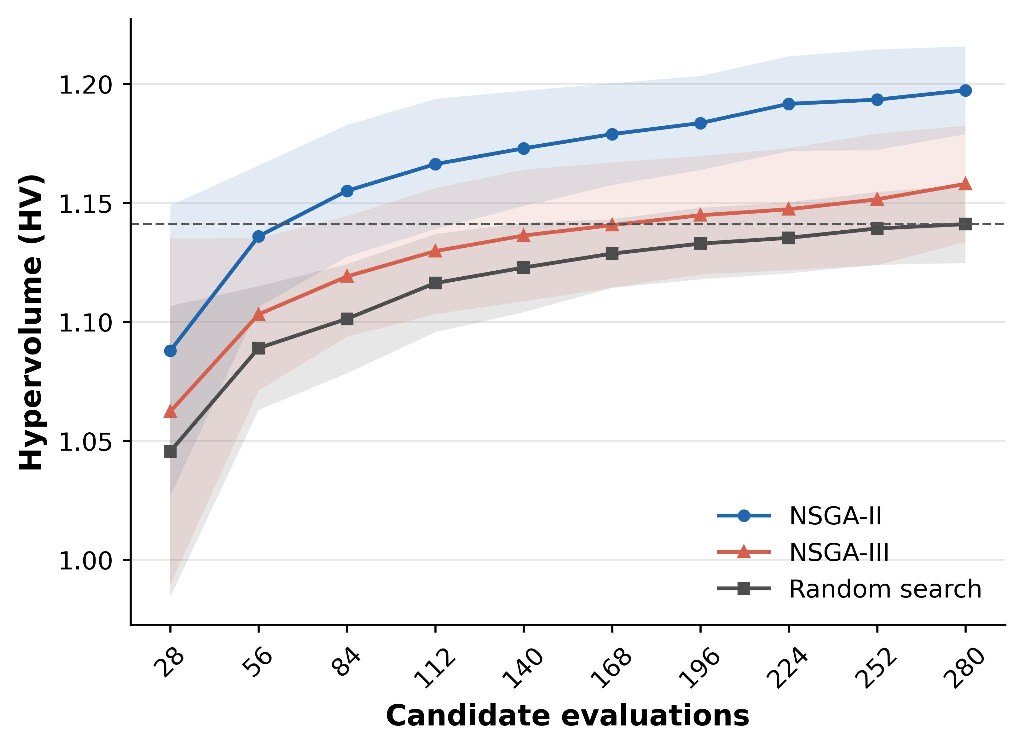
\includegraphics[width=\linewidth]
        {figures/fig_optimizer_convergence.pdf}
        \caption{Convergence of NSGA-II, NSGA-III, and matched-budget random search over 280 unique candidate evaluations. Curves show the mean indicator value across 15 independent runs and shaded regions show $\pm$1 standard deviation. All methods were evaluated at the same 28-evaluation checkpoints using fixed global objective normalisation.}
        \label{fig:optimizer_convergence}
    \end{figure}
}{}

Taken together, the results identify the main search-level difference as proximity to a stronger error--parameter--latency trade-off surface. NSGA-II consistently achieved higher hypervolume than both alternatives and lower distance-based indicators than random search. The comparison with NSGA-III was clearest for hypervolume, IGD$^{+}$, and LOO-IGD, whereas conventional IGD alone did not establish a significant pairwise difference between the two evolutionary methods. This distinction is retained rather than reducing the comparison to a single indicator.

% =========================================================
% 5.3 EVALUATION BUDGET REQUIRED TO REACH EQUIVALENT
%     FRONT QUALITY
% =========================================================

\subsection{Evaluation Budget Required to Reach Equivalent Front Quality}
\label{sec:budget_parity}

Final hypervolume describes approximation-front quality after the complete search budget, but it does not indicate how quickly that level of quality was reached. A complementary analysis therefore measured the number of candidate evaluations required for each run to attain the final mean hypervolume achieved by random search after 280 evaluations. The target hypervolume was fixed at

\begin{equation}
\mathrm{HV}_{\mathrm{target}} = 1.141019.
\label{eq:hv_parity_threshold}
\end{equation}

For search method $m$ and run $r$, the first-passage evaluation count was defined as

\begin{equation}
e^{*}_{m,r}
=
\min
\left\{
e :
\mathrm{HV}_{m,r}(e)
\geq
\mathrm{HV}_{\mathrm{target}}
\right\}.
\label{eq:first_passage}
\end{equation}

Runs that did not attain the threshold within the 280-evaluation budget were treated as non-reachers and were not assigned an artificial first-passage value.

NSGA-II reached the target hypervolume in all 15 independent runs. Among these runs, the mean first-passage budget was 71.2 evaluations, with an SD of 49.8 evaluations. NSGA-III reached the same threshold in 10 of 15 runs and required 125.1 evaluations on average among the successful runs. Random search reached its own final mean hypervolume in only 8 of 15 runs within the allotted budget and required 166.6 evaluations on average among those runs.

Table~\ref{tab:budget_parity} summarises the first-passage results.

\begin{table}[htbp]
\centering
\caption{Evaluation budget required to reach the final mean hypervolume of random search. Mean and SD are calculated only across runs that reached the threshold; non-reaching runs were retained as censored observations.}
\label{tab:budget_parity}
\begin{tabular}{lrrrr}
\toprule
\textbf{Method} &
\textbf{Runs reaching target} &
\textbf{Mean evaluations} &
\textbf{SD} &
\textbf{Relative evaluation cost} \\
\midrule
NSGA-II &
15/15 &
71.2 &
49.8 &
0.427 \\

NSGA-III &
10/15 &
125.1 &
67.0 &
0.751 \\

Random search &
8/15 &
166.6 &
68.0 &
1.000 \\
\bottomrule
\end{tabular}
\end{table}

Among the runs that reached the threshold, NSGA-II required approximately 2.34 times fewer candidate evaluations than random search to attain the same front-quality level. NSGA-III required approximately 1.33 times fewer evaluations than random search among the corresponding successful runs.

The reach rates provide an additional distinction that is not captured by the mean first-passage budget alone. Every NSGA-II run crossed the threshold within the available budget, whereas five NSGA-III runs and seven random-search runs did not. The 2.34-fold comparison should therefore be interpreted only among successful runs rather than as a complete uncensored speed ratio between the methods.

\IfFileExists{figures/fig_budget_to_parity.pdf}{
    The first-passage budgets and censored runs are visualised in Figure~\ref{fig:budget_to_parity}.

    \begin{figure}[htbp]
        \centering
        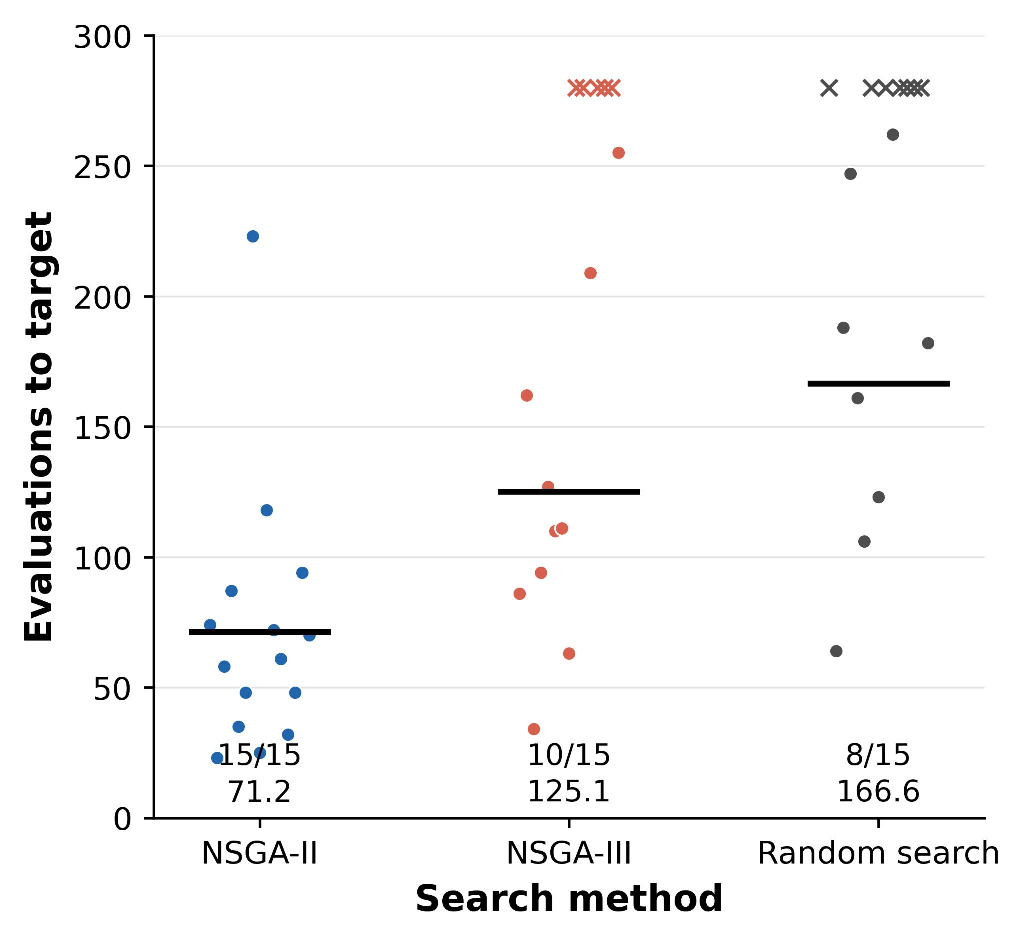
\includegraphics[width=\linewidth]
        {figures/fig_budget_to_parity.pdf}
        \caption{Candidate evaluations required to reach the final mean hypervolume of random search ($\mathrm{HV}=1.141019$). Each point represents one independent search run. Runs that did not reach the threshold within 280 evaluations are shown as censored at the evaluation limit rather than assigned an imputed first-passage value.}
        \label{fig:budget_to_parity}
    \end{figure}
}{}

The result indicates that the principal benefit of NSGA-II appeared in search efficiency rather than in a large reduction in the best prediction error. It reached a comparable error--parameter--latency trade-off surface using substantially fewer trained candidate models and reached that level in every independent run. This distinction is important for neural hyperparameter optimisation because each candidate evaluation required complete model training and recursive validation.

% =========================================================
% 5.4 FRONT CARDINALITY, SPACING, AND POOLED
%     PARETO-FRONT COMPOSITION
% =========================================================

\subsection{Front Cardinality, Spacing, and Pooled Pareto-Front Composition}
\label{sec:front_structure}

The improvement in front-quality indicators reported in Section~\ref{sec:optimizer_results} could arise for several reasons. An optimiser may return more nondominated solutions, distribute them more evenly across objective space, place them closer to the best-known trade-off surface, or combine these effects. Front cardinality and Schott spacing were therefore examined separately from hypervolume and IGD.

The mean number of nondominated solutions at the final 280-evaluation checkpoint was similar for all three search methods. NSGA-II produced $20.73\pm5.39$ nondominated solutions per run, NSGA-III produced $21.13\pm4.57$, and random search produced $21.47\pm4.34$. The Kruskal--Wallis comparison did not indicate a difference in front cardinality ($H=0.137$, $p=0.934$).

Schott spacing showed the same pattern. Mean spacing was $0.0840\pm0.0618$ for NSGA-II, $0.0824\pm0.0499$ for NSGA-III, and $0.0703\pm0.0437$ for random search. The overall comparison was not statistically significant ($H=0.040$, $p=0.980$). All Holm-adjusted pairwise comparisons for both front cardinality and spacing yielded $p=1.0$.

Table~\ref{tab:front_structure} summarises these results.

\begin{table}[htbp]
\centering
\caption{Final approximation-set cardinality and Schott spacing after 280 evaluations. Values are mean $\pm$ standard deviation across 15 independent runs. Smaller spacing indicates more even local separation of nondominated solutions \cite{schott1995spacing}.}
\label{tab:front_structure}
\begin{tabular}{lcc}
\toprule
\textbf{Method} &
\textbf{Front size} &
\textbf{Schott spacing} \\
\midrule
NSGA-II &
$20.733 \pm 5.391$ &
$0.0840 \pm 0.0618$ \\

NSGA-III &
$21.133 \pm 4.565$ &
$0.0824 \pm 0.0499$ \\

Random search &
$21.467 \pm 4.340$ &
$0.0703 \pm 0.0437$ \\
\midrule
Kruskal--Wallis $p$ &
0.934 &
0.980 \\
\bottomrule
\end{tabular}
\end{table}

The absence of a detectable difference in either quantity narrows the interpretation of the earlier hypervolume result. NSGA-II did not attain higher hypervolume by returning a larger final approximation set, nor was its advantage associated with more uniform local spacing. Instead, its nondominated solutions occupied more favourable regions of the error--parameter--latency objective space and lay closer to the best-known trade-off surface.

A second view was obtained by pooling all 12,600 candidate evaluations and extracting the global nondominated set. This procedure produced 28 solutions. Of these, 21 originated from NSGA-II, five from random search, and two from NSGA-III, as summarised in Table~\ref{tab:pooled_front}.

\begin{table}[htbp]
\centering
\caption{Method contribution to the pooled nondominated set obtained from all 12,600 search evaluations.}
\label{tab:pooled_front}
\begin{tabular}{lrr}
\toprule
\textbf{Method} &
\textbf{Pooled nondominated points} &
\textbf{Share (\%)} \\
\midrule
NSGA-II &
21 &
75.0 \\

Random search &
5 &
17.9 \\

NSGA-III &
2 &
7.1 \\
\midrule
Total &
28 &
100.0 \\
\bottomrule
\end{tabular}
\end{table}

The pooled-front composition does not conflict with the similar per-run front sizes in Table~\ref{tab:front_structure}. Each method typically returned approximately 21 nondominated solutions within an individual run, but many of those solutions became dominated when candidates from all methods and runs were compared together. NSGA-II accounted for three quarters of the solutions that remained nondominated after this global comparison.

\IfFileExists{figures/fig_pooled_pareto_front.pdf}{
    The pooled trade-off structure is shown in pairwise objective projections in Figure~\ref{fig:pooled_pareto_front}.

    \begin{figure}[htbp]
        \centering
        
\includegraphics[width=\linewidth]
        {figures/fig_pooled_pareto_front.pdf}
        \caption{Pooled multi-objective search results across all 12,600 candidate evaluations. Pairwise projections show validation rollout macro MAPE, trainable parameter count, and inference latency in the transformed objective space. The globally nondominated solutions are distinguished by the search method that produced them.}
        \label{fig:pooled_pareto_front}
    \end{figure}
}{}

Taken together, the cardinality, spacing, and pooled-front analyses indicate that the NSGA-II advantage was principally one of convergence toward higher-quality trade-offs rather than greater front size or more even within-front diversity. This interpretation is consistent with the higher hypervolume, lower IGD$^{+}$ and leave-one-method-out IGD, and lower evaluation budget required to reach the random-search reference level.

% =========================================================
% 5.5 BEST-FOUND PREDICTION ERROR AND THE LIMITS OF
%     SINGLE-RUN WINNERS
% =========================================================

\subsection{Best-Found Prediction Error and the Limits of Single-Run Winners}
\label{sec:best_found_error}

The ranking obtained from Pareto-front indicators was not reproduced when each search run was reduced to its single lowest validation macro MAPE. The mean per-run minimum was 0.9518\% for NSGA-II, 0.9486\% for NSGA-III, and 0.9637\% for random search. Their distributions overlapped substantially, as shown in Table~\ref{tab:best_found_mape}.

\begin{table}[htbp]
\centering
\caption{Best recursive validation macro MAPE observed within each independent search run. Values summarise the 15 run-wise minima for each method.}
\label{tab:best_found_mape}
\begin{tabular}{lrrrrr}
\toprule
\textbf{Method} &
\textbf{Mean (\%)} &
\textbf{SD (pp)} &
\textbf{Median (\%)} &
\textbf{Minimum (\%)} &
\textbf{Maximum (\%)} \\
\midrule
NSGA-II &
0.9518 &
0.0759 &
0.9633 &
0.8398 &
1.1147 \\

NSGA-III &
0.9486 &
0.0893 &
0.9256 &
0.8398 &
1.1226 \\

Random search &
0.9637 &
0.1076 &
0.9707 &
0.7309 &
1.1356 \\
\bottomrule
\end{tabular}
\end{table}

The single lowest search-stage value, 0.7309\%, was obtained by random search rather than by either evolutionary method. NSGA-II and NSGA-III both reached minima of 0.8398\%. Consequently, a comparison based only on the smallest prediction error observed during optimisation would not support the front-quality ranking reported in Sections~\ref{sec:optimizer_results} and~\ref{sec:budget_parity}.

This difference arises because the search objectives were explicitly multi-objective. A candidate with the smallest validation error can still be dominated or weakly positioned when parameter count and inference latency are considered jointly. Conversely, a method can produce a stronger approximation front without producing the lowest isolated MAPE value encountered anywhere in the search. The higher hypervolume and lower distance-based indicators obtained by NSGA-II therefore reflect the quality of the complete error--complexity--latency trade-off set rather than superiority of one extreme accuracy-oriented candidate.

The run-wise minima also require caution because each is selected from 280 stochastic neural-network evaluations. Section~\ref{sec:noise_results} showed that repeated training of a fixed configuration produced macro-MAPE standard deviations of 0.21--0.52~pp. Selecting the minimum from many such noisy evaluations can therefore yield an optimistic estimate of the expected performance of the corresponding configuration.

A direct paired estimate of this selection effect was not available. None of the 45 exact run-winning candidate identifiers appeared in the independently retrained noise-floor or re-screening panels. An exact candidate-matched comparison between search-stage minima and multi-seed retraining was therefore not possible, and no approximate candidate matching was substituted.

The available evidence is instead descriptive. Mean per-run search minima were approximately 0.95\%, whereas the ten-seed means of the fixed noise-floor configurations ranged from 1.55\% to 3.26\%, and the independently re-screened candidate means ranged from approximately 1.95\% to 3.51\%. These groups contain different configurations and should not be interpreted as a measured ``optimism gap''. They nevertheless show why the minimum value observed during a large stochastic search was not treated as the expected performance of the final model.

For this reason, best-found validation MAPE was used only as a descriptive search statistic. Claims about optimiser performance were based on repeated-run Pareto-front indicators, while claims about selected forecasting configurations were deferred to the independent multi-seed confirmation stage.

% =========================================================
% 5.6 MULTI-SEED CONFIRMATION OF SELECTED CONFIGURATIONS
% =========================================================

\subsection{Multi-Seed Confirmation of the Selected Configurations}
\label{sec:final_confirmation_results}

The final comparison did not reproduce the search-level separation between the optimisation methods. All three search procedures ultimately selected the same compact architecture class: a single-layer LSTM with 64 hidden units and 36,418 trainable parameters. The selected configurations differed only in sequence length, rollout horizon, and learning rate. Consequently, the final-model comparison cannot be used to distinguish the optimisation algorithms themselves; that distinction is supported by the repeated-run Pareto-front results in Sections~\ref{sec:optimizer_results}--\ref{sec:front_structure}.

The configurations subjected to ten-seed confirmation are listed in Table~\ref{tab:final_configs}. The manually specified reference contained 486,978 parameters, whereas each optimiser-selected model contained 36,418 parameters.

\begin{table}[htbp]
\centering
\caption{Configurations retained for ten-seed final confirmation.}
\label{tab:final_configs}
\begin{tabular}{lrrrrrr}
\toprule
\textbf{Configuration} &
\textbf{$L$} &
\textbf{$d_h$} &
\textbf{Layers} &
\textbf{$H$} &
\textbf{Learning rate} &
\textbf{Parameters} \\
\midrule
Manual &
20 & 192 & 2 & 8 &
0.001000000 &
486,978 \\

NSGA-II &
15 & 64 & 1 & 8 &
0.001215422 &
36,418 \\

NSGA-III &
20 & 64 & 1 & 8 &
0.000868730 &
36,418 \\

Random search &
15 & 64 & 1 & 5 &
0.000739324 &
36,418 \\
\bottomrule
\end{tabular}
\end{table}

Across the ten confirmation seeds, the NSGA-II finalist attained the lowest mean macro MAPE at 1.8097\%, followed by the manual configuration at 1.8559\%, random search at 1.8622\%, and NSGA-III at 1.8716\%. The differences were small relative to the seed-to-seed variation. The 95\% confidence intervals overlapped substantially for all four configurations.

\begin{table}[htbp]
\centering
\caption{Ten-seed held-out performance of the manually specified and optimiser-selected configurations. Values are calculated on the common 76-point recursive test window.}
\label{tab:final_accuracy}
\begin{tabular}{lrrrr}
\toprule
\textbf{Configuration} &
\textbf{Macro MAPE (\%)} &
\textbf{SD (pp)} &
\textbf{95\% CI} &
\textbf{$Q$ / $R_e$ MAPE (\%)} \\
\midrule
Manual &
1.8559 &
0.2270 &
[1.7229, 1.9921] &
2.8466 / 0.8651 \\

NSGA-II &
1.8097 &
0.3716 &
[1.5764, 2.0107] &
2.8147 / 0.8048 \\

NSGA-III &
1.8716 &
0.3494 &
[1.6387, 2.0533] &
2.6918 / 1.0514 \\

Random search &
1.8622 &
0.1554 &
[1.7685, 1.9485] &
2.8970 / 0.8274 \\
\bottomrule
\end{tabular}
\end{table}

The mean difference between the NSGA-II finalist and the manual reference was $-0.0461$ percentage points, with a 95\% bootstrap confidence interval of $[-0.3836,\,0.2293]$ percentage points. The paired Wilcoxon test gave a raw $p$-value of 0.7695, and the Holm-adjusted value was 1.0. The corresponding comparisons of the NSGA-III and random-search finalists with the manual configuration were also non-significant. After correction, all three optimiser-selected configurations had $p=1.0$ for the macro-MAPE comparison.

The numerically lower mean obtained by NSGA-II should therefore not be interpreted as an improvement in predictive accuracy. The ten-seed experiment detected no statistically significant accuracy difference between the NSGA-II finalist and the manually specified reference. The confidence interval was also too wide to establish practical equivalence within a narrow error margin.

The resource differences were considerably larger than the accuracy differences. Each optimiser-selected configuration contained 92.5\% fewer trainable parameters than the manual reference. Mean batch-one forward latency decreased from 0.696~ms for the manual model to approximately 0.413--0.425~ms for the compact finalists. Recorded final-training time was also lower for all three selected models.

\begin{table}[htbp]
\centering
\caption{Computational characteristics of the confirmed configurations. Forward latency was measured under the common Tesla T4 protocol. Training time denotes recorded model-training time for the final training schedule.}
\label{tab:final_compute}
\begin{tabular}{lrrr}
\toprule
\textbf{Configuration} &
\textbf{Parameters} &
\textbf{Forward latency (ms)} &
\textbf{Training time (s)} \\
\midrule
Manual &
486,978 &
$0.6956 \pm 0.0014$ &
$16.482 \pm 2.869$ \\

NSGA-II &
36,418 &
$0.4248 \pm 0.0202$ &
$6.227 \pm 0.452$ \\

NSGA-III &
36,418 &
$0.4219 \pm 0.0158$ &
$4.690 \pm 0.336$ \\

Random search &
36,418 &
$0.4130 \pm 0.0175$ &
$6.461 \pm 0.291$ \\
\bottomrule
\end{tabular}
\end{table}

Table~\ref{tab:final_compute} shows the corresponding computational characteristics. Relative to the manual configuration, the NSGA-II finalist reduced forward-pass latency by 38.9\% and recorded training time by 62.2\%. Its complete recursive-trajectory latency was 35.3\% lower. The corresponding trajectory-latency reductions were 38.0\% for NSGA-III and 36.2\% for random search. These reductions accompanied a 92.5\% decrease in parameter count for all three optimiser-selected models.

Seed-to-seed error dispersion varied numerically across the configurations. Macro-MAPE SD was 0.2270~pp for the manual model, 0.3716~pp for NSGA-II, 0.3494~pp for NSGA-III, and 0.1554~pp for random search. However, neither Levene's test ($p=0.1316$) nor the Brown--Forsythe test ($p=0.3134$) rejected equality of variance. The larger numerical dispersion of the NSGA-II and NSGA-III finalists was therefore treated as descriptive rather than as evidence that compact models were less stable.

These results separate two conclusions that would otherwise be easy to conflate. At the search level, NSGA-II converged more consistently toward stronger multi-objective fronts under the matched evaluation budget. At the final-model level, however, the three search methods selected similarly compact LSTM architectures, and no statistically significant improvement in held-out prediction error over the manual reference was detected. The practical gain of the selected NSGA-II model was therefore primarily a reduction in model size and computational demand rather than a demonstrated increase in predictive accuracy.

% =========================================================
% 5.7 SENSITIVITY TO THE FINAL SELECTION RULE
% =========================================================

\subsection{Sensitivity to the Final Selection Rule}
\label{sec:selection_sensitivity}

The final configuration associated with each search method depended on the decision rule applied after three-seed re-screening. The implemented rule balanced re-screened macro MAPE, parameter count, and latency through the normalised Euclidean distance to the ideal point described in Section~\ref{sec:final_selection}. To examine whether this choice materially affected the reported finalists, the knee-selected configuration was compared with a purely accuracy-prioritised alternative.

For NSGA-II and random search, the two rules selected the same configuration. The lowest re-screened MAPE for NSGA-II was obtained by the $L=15$, $d_h=64$, one-layer, $H=8$ candidate with 36,418 parameters, which was also selected by the implemented knee rule. Random search showed the same agreement for its $L=15$, $d_h=64$, one-layer, $H=5$ candidate.

NSGA-III was the only method for which the selection rule changed the retained configuration. Its lowest re-screened MAPE was obtained by a larger model with $L=15$, $d_h=96$, one LSTM layer, and $H=3$. This candidate contained 62,658 parameters and achieved a three-seed re-screened macro MAPE of $1.9489\pm0.1416$\%. The implemented knee rule instead selected the $L=20$, $d_h=64$, one-layer, $H=8$ configuration with 36,418 parameters and a re-screened macro MAPE of $2.2853\pm0.0983$\%.

Table~\ref{tab:selection_sensitivity} summarises the comparison.

\begin{table}[htbp]
\centering
\caption{Sensitivity of finalist selection to the post-search decision rule. Re-screened MAPE values are mean $\pm$ standard deviation over seeds 42, 52, and 62.}
\label{tab:selection_sensitivity}
\begin{tabular}{llll}
\toprule
\textbf{Method} &
\textbf{Accuracy-priority candidate} &
\textbf{Implemented knee candidate} &
\textbf{Same selection?} \\
\midrule

NSGA-II &
\begin{tabular}[c]{@{}l@{}}
$L15\_D64\_N1\_H8$ \\
$2.3275\pm0.4095$\%, 36,418 params
\end{tabular}
&
\begin{tabular}[c]{@{}l@{}}
$L15\_D64\_N1\_H8$ \\
$2.3275\pm0.4095$\%, 36,418 params
\end{tabular}
&
Yes \\[2mm]

NSGA-III &
\begin{tabular}[c]{@{}l@{}}
$L15\_D96\_N1\_H3$ \\
$1.9489\pm0.1416$\%, 62,658 params
\end{tabular}
&
\begin{tabular}[c]{@{}l@{}}
$L20\_D64\_N1\_H8$ \\
$2.2853\pm0.0983$\%, 36,418 params
\end{tabular}
&
No \\[2mm]

Random search &
\begin{tabular}[c]{@{}l@{}}
$L15\_D64\_N1\_H5$ \\
$2.4432\pm0.4458$\%, 36,418 params
\end{tabular}
&
\begin{tabular}[c]{@{}l@{}}
$L15\_D64\_N1\_H5$ \\
$2.4432\pm0.4458$\%, 36,418 params
\end{tabular}
&
Yes \\
\bottomrule
\end{tabular}
\end{table}

For NSGA-III, the resource-aware rule therefore accepted a re-screened MAPE increase of approximately 0.34 percentage points in exchange for a reduction from 62,658 to 36,418 parameters, corresponding to approximately 41.9\% fewer trainable parameters. This was a consequence of the stated three-objective decision rule rather than a failure to identify the lower-error candidate.

The sensitivity analysis also places the final ten-seed comparison in context. The reported NSGA-III finalist in Section~\ref{sec:final_confirmation_results} is the resource-aware knee configuration, not the lowest-error re-screened NSGA-III candidate. The accuracy-priority candidate was evaluated over only the three re-screening seeds and did not undergo the ten-seed final-confirmation experiment. Its $1.9489\%$ result should therefore not be compared directly with the ten-seed means reported in Table~\ref{tab:final_accuracy} as though both estimates had the same level of replication.

The effect of the selection rule was thus limited to one of the three search methods. For NSGA-II and random search, accuracy-priority and multi-objective knee selection coincided. For NSGA-III, the implemented decision rule deliberately favoured the smaller model. This sensitivity should be considered when interpreting the apparent similarity of the three 36,418-parameter finalists: convergence to that common model size was partly a consequence of the resource-aware post-search decision rule rather than evidence that all three search processes identified exactly the same accuracy-oriented solution.

% =========================================================
% 5.8 TEACHER-FORCED VERSUS RECURSIVE FEATURE ABLATION
% =========================================================

\subsection{Teacher-Forced Versus Recursive Feature Ablation}
\label{sec:feature_ablation_results}

The feature-ablation results depended strongly on the forecasting protocol. Under teacher-forced evaluation, several compact feature subsets appeared to outperform the full input representation. These conclusions changed once the same variants were evaluated recursively, where predicted target values were fed back into subsequent input windows.

Table~\ref{tab:feature_ablation_results} reports macro MAPE under both protocols. The full-feature baseline obtained 1.168\% under teacher forcing and 1.457\% under recursive rollout. Removing temperature increased MAPE to 1.312\% under teacher forcing and 2.004\% under rollout, while removing the ageing index produced corresponding values of 1.374\% and 1.847\%.

\begin{table}[htbp]
\centering
\caption{Feature-ablation performance under teacher-forced and recursive-rollout evaluation. Lower macro MAPE is preferred. Rankings were calculated separately within each evaluation protocol.}
\label{tab:feature_ablation_results}
\small
\begin{tabular}{lrrrr}
\toprule
\textbf{Feature set} &
\textbf{Teacher MAPE (\%)} &
\textbf{Rank} &
\textbf{Rollout MAPE (\%)} &
\textbf{Rank} \\
\midrule
Full feature set
& 1.168 & 5 & 1.457 & 3 \\

No temperature
& 1.312 & 6 & 2.004 & 6 \\

No ageing index
& 1.374 & 7 & 1.847 & 4 \\

$k_{\mathrm{exp}} + T$
& \textbf{0.613} & \textbf{1} & 1.938 & 5 \\

$k_{\mathrm{exp}} + R_{e,0}$
& 0.616 & 2 & \textbf{1.284} & \textbf{1} \\

$k_{\mathrm{exp}} + T + R_{e,0}$
& 0.682 & 3 & 2.090 & 7 \\

$k_{\mathrm{exp}} + T + R_{e,0}
 + R_{\mathrm{pulse},0} + Q_0$
& 0.806 & 4 & 1.406 & 2 \\
\bottomrule
\end{tabular}
\end{table}

The strongest contrast occurred for the compact input sets. The combination $k_{\mathrm{exp}}+T$ achieved the lowest teacher-forced MAPE, at 0.613\%, but its error increased to 1.938\% under recursive rollout, placing it fifth among the seven variants. In contrast, $k_{\mathrm{exp}}+R_{e,0}$ achieved a nearly identical teacher-forced error of 0.616\% but retained substantially better recursive performance, with the lowest rollout MAPE of 1.284\%.

Adding temperature to this compact representation did not improve recursive forecasting. The $k_{\mathrm{exp}}+T+R_{e,0}$ variant achieved 0.682\% under teacher forcing but deteriorated to 2.090\% under rollout, the highest recursive error among the tested variants. By comparison, the five-variable subset containing $k_{\mathrm{exp}}$, $T$, $R_{e,0}$, $R_{\mathrm{pulse},0}$, and $Q_0$ obtained 1.406\% under rollout and ranked second.

\IfFileExists{figures/fig_teacher_rollout_ablation.pdf}{
    The rank changes are visualised in Figure~\ref{fig:teacher_rollout_ablation}.

    \begin{figure}[htbp]
        \centering
        
\includegraphics[width=\linewidth]
        {figures/fig_teacher_rollout_ablation.pdf}
        \caption{Change in macro MAPE between teacher-forced and recursive-rollout evaluation for the feature-ablation variants. Lower values indicate better prediction. Several feature sets that appeared favourable under teacher forcing changed markedly in rank when predictions were propagated recursively.}
        \label{fig:teacher_rollout_ablation}
    \end{figure}
}{}

The disagreement between the two evaluation protocols can be explained by their different information structures. During teacher forcing, the model repeatedly receives measured target history when forming the next prediction. Errors therefore do not propagate through the subsequent sequence. Under recursive rollout, previous predictions replace the corresponding measured target values, allowing local errors and feature deficiencies to influence later forecast steps. A compact feature set that performs well when repeatedly anchored by observations is therefore not necessarily the feature set that best supports autonomous multi-step forecasting.

The $k_{\mathrm{exp}}+R_{e,0}$ result is particularly relevant in this respect. Despite using only two exogenous descriptors in addition to the required target-history channels, it produced the lowest recursive MAPE among the tested ablations. The result indicates that a larger input set was not automatically advantageous under recursive deployment. It does not, however, establish that these two variables constitute a universally optimal battery representation; the finding is specific to the present dataset, prediction targets, and rollout protocol.

The ablation results also clarify why feature selection based exclusively on teacher-forced error can be misleading for recursive degradation forecasting. Under teacher forcing, $k_{\mathrm{exp}}+T$ would have been selected as the best-performing subset. Under the deployment-aligned recursive protocol, the same choice would have produced 1.938\% MAPE rather than the 1.284\% achieved by $k_{\mathrm{exp}}+R_{e,0}$. Feature-ablation conclusions were therefore evaluated using the same rollout conditions intended for final forecasting rather than inferred from one-step prediction alone.

% =========================================================
% 5.9 EFFECT OF THE ARRHENIUS-DERIVED STRESS FEATURE
% =========================================================

\subsection{Effect of the Arrhenius-Derived Stress Feature}
\label{sec:stress_results}

Adding the Arrhenius-derived stress descriptor consistently reduced recursive forecasting accuracy. The four-feature base model obtained a macro MAPE of $2.587\pm0.341$\%, whereas the otherwise matched model containing the additional stress channel obtained $3.210\pm0.434$\%. The mean deterioration was therefore 0.623 percentage points.

The direction of the effect was consistent across all ten matched training seeds. Macro MAPE increased for every seed after the stress descriptor was added, and the paired Wilcoxon signed-rank test confirmed a statistically significant difference ($p=0.001953$). Because the two models used matched initialisation, the observed change was not attributable to independently sampled starting weights.

\begin{table}[htbp]
\centering
\caption{Effect of adding the Arrhenius-derived stress descriptor. Values are mean $\pm$ standard deviation across ten matched training seeds.}
\label{tab:stress_results}
\begin{tabular}{lccc}
\toprule
\textbf{Variant} &
\textbf{Macro MAPE (\%)} &
\textbf{$Q$ MAPE (\%)} &
\textbf{$R_e$ MAPE (\%)} \\
\midrule
Base representation &
$2.587 \pm 0.341$ &
$3.360 \pm 0.436$ &
$1.814 \pm 0.641$ \\

Base + $S_{\mathrm{Arr}}$ &
$3.210 \pm 0.434$ &
$3.655 \pm 0.469$ &
$2.764 \pm 0.508$ \\
\bottomrule
\end{tabular}
\end{table}

Table~\ref{tab:stress_results} shows that the deterioration was larger for resistance prediction than for capacity prediction. Adding the descriptor increased capacity MAPE by approximately 0.30 percentage points, whereas resistance MAPE increased by approximately 0.95 percentage points. These target-specific differences are descriptive because separate hypothesis tests were not performed for the two target errors.

The negative result can be interpreted from the construction of the descriptor,

\begin{equation}
S_{\mathrm{Arr}}
=
\ln\!\left[\max(k_{\mathrm{exp}},10^{-6})\right]
-
\frac{E_a}{RT}.
\label{eq:stress_result_definition}
\end{equation}

Two of its principal quantities, $k_{\mathrm{exp}}$ and temperature, were already supplied directly to the forecasting model. The fitted activation energy also occupied a comparatively narrow range across the source cells, from \(51.75\) to \(61.48~\mathrm{kJ\,mol^{-1}}\), with a mean of \(55.69\pm2.86~\mathrm{kJ\,mol^{-1}}\). The added channel therefore contained a nonlinear transformation of information that was already largely available to the network rather than an independent measurement.

A second issue arose at the beginning-of-life boundary. When $k_{\mathrm{exp}}=0$, the logarithmic term was evaluated after clipping the input to $10^{-6}$, giving $\ln(10^{-6})=-13.82$. At $k_{\mathrm{exp}}=1$, the corresponding logarithmic contribution is zero. The transformation therefore introduced a 13.82-unit discontinuity between these two ageing-index values. The archived minimum stress value of $-38.3374$ was reproduced by this clipping operation at $0\,^{\circ}\mathrm{C}$ with the mean fitted activation energy. No frequency claim is made here for the affected beginning-of-life records because their exact archived count has not been recovered.

The activation-energy term also differed from an independently measured physical input. It was obtained from a fit to capacity-fade data and was subsequently merged into the sequence representation. The stress channel should therefore be interpreted as a derived, model-based descriptor rather than as an additional measured operating variable.

Taken together, the matched-seed result indicates that physical motivation alone did not make the constructed descriptor useful for recursive prediction. In this formulation, the stress variable added information that was largely redundant with existing inputs while also introducing a sharp boundary transformation. Its inclusion worsened macro MAPE by 0.62 percentage points on every matched seed rather than improving the base representation.

% =========================================================
% 5.10 SEQUENCE-MODEL AND PHYSICS-INFORMED BASELINES
% =========================================================

\subsection{Sequence-Model and Physics-Informed Baselines}
\label{sec:baseline_results}

% ---------------------------------------------------------
% 5.10.1 SEQUENCE-MODEL BASELINES
% ---------------------------------------------------------

\subsubsection{Sequence-Model Baselines}
\label{sec:sequence_baseline_results}

The additional sequence architectures did not improve recursive forecasting over the compact LSTM finalists. Across five training seeds, the TCN obtained a macro MAPE of $2.088\pm0.308$\%, while the Mamba model obtained $2.945\pm0.208$\%. Their target-specific errors and parameter counts are reported in Table~\ref{tab:sequence_baseline_results}.

\begin{table}[htbp]
\centering
\caption{Recursive forecasting performance of the additional sequence-model baselines. Values are mean $\pm$ standard deviation across five training seeds.}
\label{tab:sequence_baseline_results}
\begin{tabular}{lrrrr}
\toprule
\textbf{Model} &
\textbf{Parameters} &
\textbf{Macro MAPE (\%)} &
\textbf{$Q$ MAPE (\%)} &
\textbf{$R_e$ MAPE (\%)} \\
\midrule
TCN &
119,234 &
$2.088 \pm 0.308$ &
$3.108 \pm 0.362$ &
$1.069 \pm 0.338$ \\

Mamba &
70,722 &
$2.945 \pm 0.208$ &
$4.392 \pm 0.471$ &
$1.498 \pm 0.166$ \\
\bottomrule
\end{tabular}
\end{table}

For reference, the three optimiser-selected LSTM configurations produced ten-seed macro MAPE values between 1.810\% and 1.872\% in Section~\ref{sec:final_confirmation_results}. The TCN result was therefore closer to the compact LSTM range than the Mamba result, but neither additional architecture produced a lower mean recursive error.

The difference was most pronounced for capacity prediction. The TCN obtained 3.108\% capacity MAPE and the Mamba model 4.392\%, compared with approximately 2.69--2.90\% for the confirmed compact LSTM configurations. Resistance prediction was less separated, particularly for the TCN, which obtained 1.069\% MAPE.

The result is specific to the sparse recursive setting evaluated here. The usable trajectories contained at most 29 processed checkup records, and inference required repeated feedback of predicted capacity and resistance. Under these conditions, replacing the LSTM with a causal convolutional model or a selective state-space model did not improve predictive accuracy.

Runtime was not used to rank these sequence architectures. The TCN experiments were executed on CPU and were therefore not directly comparable with the Tesla-T4 measurements of the optimised LSTM models. The Mamba experiment was executed on the Tesla T4, but the archived environment did not preserve whether the fused CUDA or reference kernel path was active. Its measured latency was therefore treated as implementation-specific rather than as a general performance characteristic of the Mamba architecture.

% ---------------------------------------------------------
% 5.10.2 PHYSICS-INFORMED BASELINE
% ---------------------------------------------------------

\subsubsection{Physics-Informed Baseline}
\label{sec:pinn_results}

Explicit physics constraints also failed to improve prediction over the corresponding data-only backbone. The data-only PINN predictor obtained a macro MAPE of $7.560\pm0.195$\%, whereas adding the monotonicity, smoothness, initial-condition, and degradation-residual terms increased the error to $8.049\pm0.294$\%.

\begin{table}[htbp]
\centering
\caption{Comparison of the matched data-only and physics-constrained PINN predictors. Values are mean $\pm$ standard deviation across repeated trainings.}
\label{tab:pinn_results}
\begin{tabular}{lc}
\toprule
\textbf{Model} &
\textbf{Macro MAPE (\%)} \\
\midrule
Data-only PINN backbone &
$7.560 \pm 0.195$ \\

Physics-constrained PINN &
$8.049 \pm 0.294$ \\
\bottomrule
\end{tabular}
\end{table}

Table~\ref{tab:pinn_results} shows that the addition of the implemented physics terms increased mean macro MAPE by approximately 0.49 percentage points. No statistical test supporting a difference between these two variants was preserved, so the comparison is reported descriptively rather than as a statistically significant deterioration. The result supports the narrower conclusion that the implemented physics constraints did not improve predictive accuracy over the same backbone.

The fitted activation-energy parameter provides additional context. The full
physics-constrained model produced a value of approximately
\(57.5~\mathrm{kJ\,mol^{-1}}\). This value lay close to the imposed prior
centre of \(56~\mathrm{kJ\,mol^{-1}}\); the prior scale was
\(7~\mathrm{kJ\,mol^{-1}}\), and the parameter was constrained to the interval
\(40\text{--}80~\mathrm{kJ\,mol^{-1}}\). Across the source-cell fits used in
subsequent feature construction, activation energy ranged from
\(51.75\) to \(61.48~\mathrm{kJ\,mol^{-1}}\), with a mean of
\(55.69 \pm 2.86~\mathrm{kJ\,mol^{-1}}\). These values are therefore
prior-guided fitted quantities and are not interpreted as independent
physical measurements.

The result also agrees with the stress-feature experiment in Section~\ref{sec:stress_results}. In both cases, introducing additional physics-derived structure did not reduce recursive forecasting error. The two experiments test different interventions---one changed the training objective and the other added a derived input---so they should not be treated as equivalent failures. Together, however, they show that physical structure was beneficial only if it added information or constraints that were useful under the actual recursive prediction protocol; physical motivation by itself was insufficient.

The broader comparison therefore favoured the compact recurrent formulation for this dataset. Neither the TCN nor Mamba improved on its recursive prediction error, and the implemented PINN constraints did not improve the matched data-only backbone. These findings do not establish a general ranking of sequence architectures or physics-informed learning methods. They define the outcome under the present sparse-checkup trajectories, feature representation, training procedure, and recursive evaluation protocol.

% =========================================================
% 5.11 GROUPED FIVE-FOLD VALIDATION
% =========================================================

\subsection{Grouped Five-Fold Validation}
\label{sec:grouped_cv_results}

The grouped five-fold analysis examined whether the relative behaviour of the forecasting variants persisted when entire cells were reassigned across different held-out partitions. The seven variants showed a clear difference in their fold-wise rank distributions. The Friedman test rejected equality of ranks across the models
($\chi^{2}=24.171$, $p=4.86\times10^{-4}$).

Table~\ref{tab:grouped_cv_ranks} reports the mean rank obtained over the five held-out folds. Lower rank indicates lower macro MAPE within a fold.

\begin{table}[htbp]
\centering
\caption{Mean ranks across the five grouped cell-wise validation folds. Rank 1 corresponds to the lowest macro MAPE within a fold.}
\label{tab:grouped_cv_ranks}
\begin{tabular}{lr}
\toprule
\textbf{Forecasting variant} &
\textbf{Mean rank} \\
\midrule
Teacher-forced LSTM &
1.40 \\

Recursive-rollout LSTM &
2.60 \\

PINN-feature:
$k_{\mathrm{exp}}+R_{e,0}+Q_0+S_{\mathrm{Arr}}$ &
3.20 \\

Sparse LSTM &
3.60 \\

PINN-feature:
$k_{\mathrm{exp}}+R_{e,0}+R_{\mathrm{pulse},0}+Q_0+S_{\mathrm{Arr}}$ &
4.20 \\

Data-only PINN &
6.00 \\

Physics-constrained PINN &
7.00 \\
\bottomrule
\end{tabular}
\end{table}

The teacher-forced LSTM had the lowest mean rank at 1.40, followed by the recursive-rollout LSTM at 2.60. The two compact PINN-derived feature models occupied intermediate positions, with mean ranks of 3.20 and 4.20, while the sparse LSTM obtained a mean rank of 3.60. The data-only and physics-constrained PINN models ranked sixth and seventh, respectively.

The rank ordering should not be interpreted as evidence of pairwise statistical superiority. With only five paired folds, the smallest attainable non-zero two-sided exact Wilcoxon signed-rank $p$-value is 0.0625. Consequently, no exact pairwise comparison could reach the conventional 0.05 threshold even before adjustment for multiple comparisons. Holm-corrected pairwise superiority claims are therefore not supported by this experiment.

The comparatively favourable rank of the teacher-forced LSTM should also be interpreted in light of the forecasting protocol. Teacher-forced prediction repeatedly receives measured target history and does not experience recursive accumulation of its own prediction errors. Its first-place mean rank therefore does not establish that teacher forcing is the preferable deployment strategy. For the intended multi-step forecasting setting, the recursive-rollout results remain the deployment-aligned evaluation.

The grouped analysis nevertheless supports two broader observations from the fixed-split experiments. First, recurrent LSTM formulations remained among the highest-ranked approaches when the held-out cell composition changed. Second, adding the implemented physics constraints did not improve the data-only PINN backbone; the physics-constrained PINN obtained the highest, and therefore least favourable, mean rank of 7.00.

These results provide evidence that the principal model-family ordering was not confined to a single fixed cell partition. At the same time, the five-fold design does not provide sufficient inferential resolution for claims about individual model pairs. The grouped experiment is therefore treated as a resampling-based robustness check rather than as a second source of pairwise superiority claims.

% =========================================================
% 5.12 EXTERNAL TRANSFER AUDIT
% =========================================================

\subsection{External Transfer Audit}
\label{sec:transfer_results}

The frozen-representation, head-only adaptation protocol produced negative
transfer on the external LG M50T dataset. Across the 40 target cells, source
pretraining increased per-cell capacity MAPE by a mean of 6.99 percentage
points relative to target-only training from scratch. The median paired
increase was 5.03 percentage points, and the bootstrap 95\% confidence
interval for the mean paired effect was
$[5.19,\,8.79]$ percentage points. The paired Wilcoxon signed-rank test gave
$W=25$ and $p=1.6\times10^{-9}$.

\begin{table}[htbp]
\centering
\caption{Paired external-transfer comparisons on the LG M50T dataset.
Positive differences indicate higher capacity MAPE for the first-listed
method. Confidence intervals were obtained from 10,000 bootstrap resamples
of the paired cell-level effects.}
\label{tab:transfer_results}
\begin{tabular}{lrrrr}
\toprule
\textbf{Comparison} &
\textbf{$n$} &
\textbf{Mean difference (pp)} &
\textbf{95\% CI (pp)} &
\textbf{$p$-value} \\
\midrule
Source transfer $-$ target only &
40 &
+6.988 &
[5.187, 8.795] &
$1.6\times10^{-9}$ \\

Source transfer $-$ square-root fade &
40 &
+6.772 &
[4.907, 8.808] &
$<1\times10^{-9}$ \\

Target only $-$ square-root fade &
20 &
$\approx -0.215$ &
$\approx[-1.024,\,0.650]$ &
$\approx0.485$ \\
\bottomrule
\end{tabular}
\end{table}

Table~\ref{tab:transfer_results} summarises the paired external comparisons. The same pattern was obtained against the analytical square-root-fade
control. Source-pretrained head adaptation increased per-cell capacity MAPE
by 6.77 percentage points, with a 95\% confidence interval of
$[4.91,\,8.81]$ percentage points ($W=16$, $p<10^{-9}$). In contrast, the
archived target-only versus square-root-fade comparison showed a mean
difference of approximately $-0.22$ percentage points, with a confidence
interval spanning zero and $p\approx0.485$. Thus, the large deterioration
was associated with reuse of the frozen source representation rather than
with a clear advantage of one of the two target-domain controls.

\IfFileExists{figures/fig_external_transfer.pdf}{
    The cell-level transfer effects are visualised in Figure~\ref{fig:external_transfer}.

    \begin{figure}[htbp]
        \centering
        
\includegraphics[width=0.88\linewidth]
        {figures/fig_external_transfer.pdf}
        \caption{External transfer audit on LG M50T 21700 cells. Paired
        cell-level capacity-MAPE differences compare the frozen
        source-representation, head-only adaptation protocol with target-only
        training. Positive values indicate deterioration after source
        pretraining.}
        \label{fig:external_transfer}
    \end{figure}
}{}

The magnitude of the transfer effect was substantially larger than the
seed-induced variation observed in the source-domain experiments. The
training-noise study produced macro-MAPE standard deviations of
0.21--0.52 percentage points for fixed configurations, whereas the mean
external deterioration relative to target-only training was 6.99 percentage
points. The external result therefore cannot reasonably be interpreted as
a small fluctuation of the same scale as ordinary source-domain retraining
variation.

Several differences between the source and target datasets provide plausible
context for this result. The optimisation dataset consisted of commercial
18650 cells and contained the source-domain ageing and operating
distributions used to learn the frozen representation. The external audit
used LG M50T 21700 cells with a different capacity scale and a distinct
experimental ageing distribution. In addition, the resistance measurements
available in the two datasets were not directly comparable, which is why the
external analysis was restricted to capacity prediction. These differences
establish a dataset and operating-distribution shift, but they do not by
themselves identify the mechanism responsible for the observed negative
transfer.

The adaptation strategy also placed a strong restriction on what could be
learned from the external calibration data. The source representation was
kept fixed, and only the prediction head was updated. A representation whose
internal features were specialised to the source trajectories could therefore
not reorganise its sequence encoding in response to the target-domain data.
By contrast, the target-only model was free to learn its representation
directly from the available target calibration records.

The result should consequently be scoped to the protocol that was actually
tested. It demonstrates significant negative transfer under
\emph{frozen-representation, head-only adaptation} from the present source
corpus to the evaluated LG M50T trajectories. Full-network fine-tuning,
partial unfreezing, representation alignment, adversarial domain adaptation,
and other transfer-learning strategies were not evaluated. The experiment
therefore does not establish that transfer learning is generally ineffective
for battery degradation forecasting.

This external audit also places the source-domain optimisation gains in
perspective. Efficient convergence to a strong Pareto front and selection of
a compact source-domain model did not guarantee that the learned
representation would remain useful after dataset shift. Model efficiency,
source-domain predictive accuracy, and cross-domain transportability are
therefore distinct properties and require separate evaluation.

% =========================================================
% 5.13 SYNTHESIS OF THE OPTIMISATION RESULTS
% =========================================================

\subsection{What the Multi-Objective Optimisation Study Shows}
\label{sec:overall_discussion}

The main effect of multi-objective evolutionary search appeared in the quality
and rate of convergence of the approximation front, not in the lowest
prediction error encountered during search. Under the same 280-evaluation
budget, NSGA-II produced the highest final hypervolume and retained its
advantage under IGD$^{+}$ and leave-one-method-out IGD. It also reached the
final mean hypervolume of random search after 71 evaluations on average and
did so in all 15 runs. Random search required 167 evaluations among the
eight runs that reached the same threshold. By contrast, the distributions
of run-wise minimum MAPE overlapped, and the lowest single search-stage error
was produced by random search. The benefit of NSGA-II was therefore
front-level convergence rather than discovery of an isolated accuracy winner.

This distinction matters because a multi-objective search should not be
judged by the smallest value of one objective. Hyperparameter configurations
were evaluated simultaneously on recursive error, parameter count, and
measured latency. The front-size and spacing results further narrowed the
interpretation: NSGA-II did not return more nondominated solutions per run
and did not produce measurably more even spacing. Its advantage arose because
its solutions occupied more favourable regions of the three-objective space.
The pooled comparison was consistent with this interpretation, with NSGA-II
contributing most of the solutions that remained nondominated after all
12,600 evaluations were compared together.

The measured training-noise floor changes how individual search winners
should be read. Retraining fixed configurations produced macro-MAPE standard
deviations of 0.21--0.52 percentage points. Differences of that order can
readily alter the ordering of two configurations evaluated once. A minimum
selected from hundreds of stochastic training runs is even more exposed to
this effect because selection itself favours unusually low realizations.
Accordingly, the search-stage winner was not treated as a final estimate of
model quality. Re-screening and ten-seed confirmation were required before
the selected configurations were compared.

This finding has implications beyond the present battery testbed.
Methodological guidance for stochastic optimisation already recommends
independent runs, non-parametric comparison, and multiplicity control
\cite{latorre2021guidelines,derrac2011nonparam}. The present experiments add
a neural-training reason for following that practice: variation exists
inside each candidate evaluation as well as between optimiser runs. When
two hyperparameter configurations differ by only a few tenths of a
percentage point after one training seed, the observed ordering is
underdetermined unless the candidate-level variation is measured. A
single-run optimiser comparison can therefore confound search behaviour
with neural-training noise even when the optimisation algorithm itself is
implemented correctly.

The ten-seed confirmation also separates search quality from final-model
accuracy. The selected NSGA-II configuration obtained a numerically lower
mean MAPE than the manual reference, but the paired difference was not
statistically significant and its confidence interval did not establish
equivalence. The defensible practical outcome was instead the 92.5\%
reduction in parameter count together with lower inference and training
cost. The compact model is therefore a consequence of the multi-objective
decision process, not evidence that NSGA-II discovered a more accurate
forecasting architecture.

The forecasting experiments show why the evaluation protocol must match the
intended use of the model. Feature rankings changed substantially between
teacher-forced and recursive evaluation. In particular, a compact input set
that was best under teacher forcing deteriorated after its own predictions
were fed back, whereas $k_{\mathrm{exp}}+R_{e,0}$ remained effective under
rollout. Teacher forcing answers whether the next prediction can be made
when measured history is repeatedly supplied. Recursive rollout answers a
different question: whether prediction remains stable when future
measurements are unavailable. Feature-selection conclusions drawn from the
first setting cannot be assumed to hold in the second.

The physics-based experiments led to a similarly restrained conclusion.
Adding the Arrhenius-derived stress descriptor increased macro MAPE by
0.62 percentage points on all ten matched seeds, while the implemented
physics constraints did not improve the matched data-only PINN backbone.
Neither result argues against the use of physical knowledge in battery
forecasting. They show that a derived physical quantity or an added physics
loss must contribute useful information under the forecasting protocol being
evaluated. In the stress-feature experiment, much of the descriptor was
constructed from variables already available to the network, and the
logarithmic transformation introduced a beginning-of-life discontinuity.
Physical motivation alone did not compensate for those properties.

The external audit places a further boundary on the source-domain results.
Under frozen-representation, head-only adaptation, source pretraining
increased per-cell capacity MAPE by 6.99 percentage points on the 40
external 21700 cells relative to target-only training. This result does not
generalise to full fine-tuning or other domain-adaptation strategies, which
were not tested. It does show that a representation selected efficiently on
the source corpus was not automatically transferable under the evaluated
adaptation rule. Source-domain front quality, model compactness, and
cross-dataset transfer are separate properties.

Taken together, the experiments support a narrower but stronger conclusion
than an accuracy-centred optimiser comparison. Under a matched neural-training
budget, NSGA-II reached higher-quality error--complexity--latency fronts more
quickly and more consistently than the alternatives. That advantage did not
translate into a statistically established improvement in final held-out
accuracy. The combination of repeated optimiser runs, measured candidate
noise, recursive evaluation, and independent multi-seed confirmation was
therefore necessary to distinguish an optimisation advantage from a
favourable single training run.
% =========================================================
% 6. LIMITATIONS AND FUTURE WORK
% =========================================================

\section{Limitations and Future Work}
\label{sec:limitations}

The present findings should be interpreted within the scope of the adopted
data, model family, and optimisation setting. The primary search was conducted
on 228 commercial lithium-ion cells using a predefined LSTM search space and
a fixed budget of 280 candidate evaluations per run. The comparison therefore
characterises the relative behaviour of NSGA-II, NSGA-III, and random search
under this experimental setting. Broader studies involving additional
multi-objective optimisers, larger datasets, and alternative sequence
architectures would help determine how consistently the observed convergence
advantage persists.

A second limitation concerns stochastic candidate evaluation. Each
search-stage configuration was trained once within an optimiser run, while the
noise-floor experiment showed that repeated training of a fixed configuration
can introduce macro-MAPE variation of several tenths of a percentage point.
The subsequent re-screening and ten-seed confirmation stages reduced the
effect of this uncertainty on final model selection, but the search process
itself still operated on noisy objective values. Future work could incorporate
adaptive replication or uncertainty-aware objective modelling so that
additional training effort is concentrated on candidates close to the
evolving Pareto front.

The resource objectives also have different levels of portability. Parameter
count is independent of hardware, whereas the latency objective was measured
on a Tesla T4 under a fixed batch-one timing protocol. The resulting latency
values are therefore suitable for comparing candidates within the present
study but should be re-measured on the intended deployment platform. In
addition, the resource-aware knee rule affected the NSGA-III finalist,
indicating that post-search preference articulation can influence which member
of a Pareto set is ultimately selected. Future studies could compare several
decision rules, including accuracy-priority and explicit resource-constrained
selection.

The physics-informed and grouped-validation experiments also define useful
directions for extension. The implemented physics constraints and
Arrhenius-derived descriptor did not improve recursive forecasting under the
present formulation, but this outcome does not preclude other forms of
physics-guided learning. The exact upstream provenance of the fitted
activation-energy values used in the archived stress-feature tables was not
preserved relative to the later data partitions; those stress-based analyses
are therefore interpreted as auxiliary rather than as fully reconstructed
leakage-audited experiments. Independently measured physical quantities,
uncertainty-aware physical parameters, and constraints acting directly on
long-horizon trajectories warrant further study. The fixed final test panel
contained 76 rollout points from 10 cells, while the grouped analysis used only
five held-out folds and was not stratified by operating condition. Larger
multi-source validation would provide stronger evidence about generalisation
across ageing regimes.

Finally, the external audit examined one independent LG M50T 21700 dataset
using frozen-representation, head-only adaptation. The observed negative
transfer therefore applies to that adaptation strategy rather than to
transfer learning in general. Partial unfreezing, full-network fine-tuning,
representation alignment, and explicit domain-adaptation methods remain to be
tested. Extending the evaluation across additional cell formats and operating
conditions would clarify whether the source-domain Pareto-front advantage
translates to more transferable forecasting models.
% =========================================================
% 7. CONCLUSION
% =========================================================

\section{Conclusion}
\label{sec:conclusion}

A repeated-run multi-objective optimisation study was conducted for recursive
battery degradation forecasting, with prediction error, model size, and
measured inference latency treated as competing objectives. Under an identical
budget of 280 candidate evaluations per run, NSGA-II produced the strongest
overall Pareto-front convergence. Its final mean hypervolume was 1.1972,
compared with 1.1579 for NSGA-III and 1.1410 for matched-budget random search,
and the advantage over both alternatives was statistically significant.
NSGA-II also reached the final mean hypervolume of random search after
71.2 evaluations on average and reached this threshold in all 15 independent
runs. The corresponding threshold was reached by only 10/15 NSGA-III runs and
8/15 random-search runs.

These gains should not be interpreted as evidence that NSGA-II discovered a
more accurate final forecasting model. The lowest individual search-stage
MAPE was obtained by random search, while repeated training of fixed
configurations showed macro-MAPE standard deviations of 0.21--0.52 percentage
points. Independent re-screening and ten-seed confirmation were therefore
needed before the selected models were compared. The final NSGA-II model
achieved a mean macro MAPE of 1.810\%, compared with 1.856\% for the manual
reference, but the difference was not statistically significant. Its clearer
advantage was computational: the selected model contained 92.5\% fewer
parameters, while the held-out accuracy difference remained statistically
non-significant.

The forecasting experiments further showed that conclusions depended on the
evaluation protocol. Feature rankings changed between teacher-forced and
recursive prediction, and an Arrhenius-derived stress descriptor increased
macro MAPE on all ten matched seeds. The implemented physics constraints also
did not improve the matched data-only predictor. Finally, frozen-
representation, head-only adaptation to 40 external LG M50T 21700 cells
produced significant negative transfer, increasing per-cell capacity MAPE by
6.99 percentage points relative to target-only training.

Overall, the principal contribution of multi-objective evolutionary search in
this setting was faster and more repeatable convergence toward useful
error--complexity--latency trade-offs rather than a statistically established
gain in final prediction accuracy. The results also show why stochastic
hyperparameter optimisation should be assessed through independent search
runs, candidate re-screening, deployment-aligned recursive evaluation, and
multi-seed confirmation rather than through a single best training result.

\section*{Data and Code Availability}

The source battery datasets are available from their original providers under
their respective terms and are not redistributed. Derived split assignments,
experiment outputs, analysis code, figure-generation code, and the automated
manuscript-value reproduction check are available at
\url{https://github.com/Simhaatt/battery-moo-recursive-forecasting}. The
version used for this article is archived at Zenodo:
\url{https://doi.org/10.5281/zenodo.22057384}.
% =========================================================
% REFERENCES
% =========================================================

\bibliographystyle{elsarticle-num-names}
\bibliography{references}

\end{document}
